A participação cidadã e a colaboração por meio de empresas de tecnologia especializadas em negócios de governança pública, conhecidas como Gov-Techs, têm se tornado cada vez mais relevantes na sociedade contemporânea. Com os avanços tecnológicos e a disseminação das redes sociais, surgiram novas formas de engajamento e interação entre cidadãos e governos. Nesse contexto, o aplicativo Colab se destaca como uma plataforma inovadora que combina elementos de redes sociais com a participação cidadã em questões relacionadas à gestão pública.

Neste capítulo, abordaremos o Colab a partir de uma perspectiva que envolve as redes sociais, e-Gov (governo eletrônico) e Gov-Techs, bem como a vigilância participativa. Analisaremos suas funcionalidades, impactos sociais, desafios e limitações, explorando o papel desempenhado pelo Colab nesse contexto dinâmico de engajamento cidadão e colaboração com as instâncias governamentais.

\section{História e Desenvolvimento}
Em 31 de dezembro de 2023, o Colab publicou a matéria \cite{2023_Colab_PAGE} que faz uma retrospectiva na celebração de 10 anos da plataforma, servindo como uma fonte primária para a história que resumiremos a seguir. O Colab foi lançado em 2013 como uma iniciativa pioneira no campo da participação cidadã digital. A plataforma foi desenvolvida pelos sócios Paulo Pandolfi e Gustavo Maia, que, inspirados por suas experiências em marketing político, perceberam a necessidade de uma ferramenta que permitisse uma maior interação entre cidadãos e governos.

O objetivo do Colab é permitir que os usuários compartilhem ideias, façam sugestões, denunciem problemas e participem ativamente na construção de políticas públicas. Funcionando como uma rede social, os cidadãos podem postar fotos de problemas da cidade e solicitar uma solução. As prefeituras, por sua vez, acessam essas reclamações e têm uma solução de tecnologia em nuvem para dar andamento às solicitações.

Desde o seu lançamento, o Colab tem conquistado espaço em diversas cidades, tornando-se uma ferramenta de referência no campo da democracia digital. A plataforma foi eleita “o melhor app urbano do mundo” pela NewCities Foundation e hoje conta com 200 mil cadastros e contratos com diversas cidades, incluindo Recife, Ipojuca, Niterói, Mesquita, Maceió, Aracaju, Cruz Alta, Santo André e Juiz de Fora.

Além disso, desde 2016, o Colab também oferece uma ferramenta para que as prefeituras abram consultas sobre questões da cidade, auxiliando na tomada de decisões e na coleta de dados. Essa ferramenta tem vários formatos e gera muitos dados que ajudam a fazer uma gestão melhor com a participação do cidadão.

A história do Colab é marcada por desafios e inovações. Quando foi lançado, o aplicativo não tinha nenhuma prefeitura cadastrada. As necessidades dos cidadãos eram coletadas pela empresa e enviadas para a administração pública pelos canais de atendimento tradicionais, como site e email. No entanto, mesmo sem prefeituras cadastradas, o sistema foi reconhecido internacionalmente pela NewCities Foundation como "o melhor app urbano do mundo".

A primeira prefeitura a adotar oficialmente o Colab foi Curitiba, seguida por outras 50 no mesmo ano. Esse crescimento rápido trouxe desafios, pois a empresa precisava atender melhor e evoluir, mas ainda não tinha receita. No entanto, um contrato com a organização social Comunitas, no começo de 2015, para atender as cidades de Santos e Campinas, em São Paulo, e Pelotas, no Rio Grande do Sul, injetou dinheiro na empresa e deu ânimo aos empreendedores.

Desde a sua fundação, o Colab tem buscado desenvolver soluções tecnológicas que possam contribuir para a construção de uma gestão pública mais eficiente, transparente e participativa. Atualmente, a plataforma está presente em mais de 130 cidades, em 2 países, e conta com cerca de 900 mil usuários cadastrados.

\section{Funcionalidades}

\begin{figure}[ht]
	\centering
	\begin{subfigure}{0.33\textwidth}
		\centering
		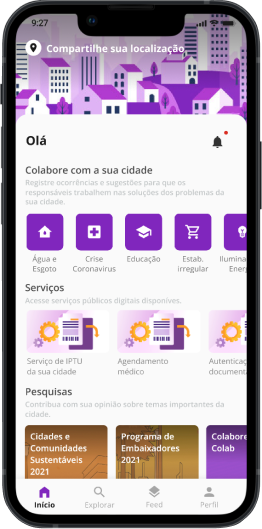
\includegraphics[width=\textwidth]{images/colab_app.png}
		\caption{Tela inicial do app}
	\end{subfigure}%
	\begin{subfigure}{0.33\textwidth}
		\centering
		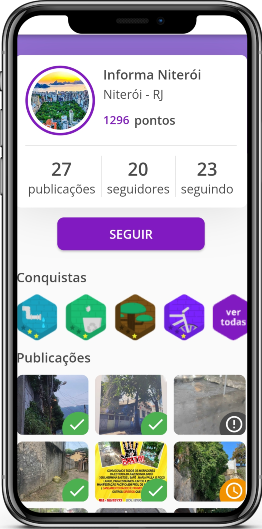
\includegraphics[width=\textwidth]{images/colab_app_perfil.png}
		\caption{Tela de perfil do usuário}
	\end{subfigure}%
	\begin{subfigure}{0.33\textwidth}
		\centering
		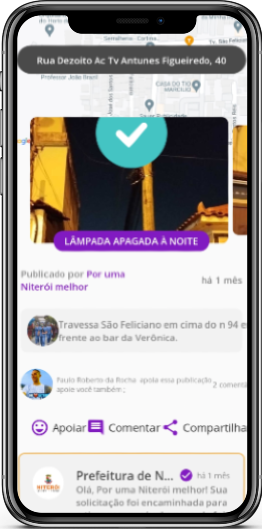
\includegraphics[width=\textwidth]{images/colab_app_evento.png}
		\caption{Tela de evento de zeladoria pública}
	\end{subfigure}
	\caption{Screenshots do aplicativo Colab}
\end{figure}

O Colab é uma plataforma digital que promove a vigilância participativa, a democracia digital e o governo eletrônico (e-Gov) por meio de uma série de funcionalidades interativas. A plataforma se destaca por permitir que os cidadãos desempenhem um papel ativo na gestão pública, contribuindo com ideias, sugestões e denúncias, e participando de consultas públicas.

A funcionalidade de publicação de ideias e sugestões permite que os usuários compartilhem suas ideias sobre questões de interesse público, abrangendo uma variedade de temas, desde melhorias na infraestrutura urbana até propostas de políticas sociais. Essa funcionalidade promove a democracia digital, permitindo que os cidadãos participem ativamente na formulação de políticas públicas.

A funcionalidade de denúncia de problemas permite que os usuários denunciem problemas como buracos nas vias, iluminação pública deficiente, entre outros. Essas denúncias são georreferenciadas, facilitando a identificação e resolução dos problemas pelas autoridades competentes. Isso contribui para a vigilância participativa, pois permite que os cidadãos monitorem a qualidade dos serviços públicos e infraestruturas em suas comunidades.

O Colab também possui uma forte componente social. Os usuários podem seguir outros usuários, serem seguidos, curtir e comentar as publicações. Isso promove a formação de uma rede social dentro do Colab, ampliando as possibilidades de engajamento e diálogo entre os participantes.

Os usuários também podem acompanhar o andamento das demandas e propostas que foram apresentadas. Isso permite que eles estejam cientes das ações tomadas pelo governo em resposta às suas contribuições, promovendo a transparência e a responsabilidade no governo eletrônico.

Além disso, o Colab introduziu recentemente novas funcionalidades, como micro consultas, reportar comentários e priorização de comentários. As micro consultas permitem que os usuários respondam perguntas rápidas do tipo sim/não diretamente na notificação push, trazendo mais dinamismo e velocidade para a gestão do relacionamento entre o cidadão e a cidade. A funcionalidade de reportar comentários permite que os usuários do Colab reportem comentários uns dos outros, mantendo a qualidade e a relevância das discussões na plataforma. A priorização de comentários, também conhecida como up/down vote, permite que os usuários indiquem o quão relevante um comentário é por meio de votos, destacando as contribuições mais valiosas.

A funcionalidade de consultas públicas é uma parte essencial do Colab, permitindo que os governos interajam diretamente com os cidadãos e obtenham feedback sobre várias questões. As consultas podem ser personalizadas para se adaptarem à realidade de cada território, e os gestores públicos podem criar seus próprios processos. Além disso, é possível configurar as consultas para permitir respostas anônimas. Essa funcionalidade promove a democracia digital e o governo eletrônico, permitindo que os cidadãos participem diretamente na tomada de decisões do governo.

A gamificação é um aspecto central do Colab, usada para aumentar o engajamento dos cidadãos e incentivá-los a participar ativamente na melhoria de suas cidades. A gamificação envolve o uso de elementos de design de jogos em contextos não-jogáveis para motivar a participação, envolvimento e lealdade.

No Colab, aspectos de gamificação são implementadas através da "Jornada do Cidadão", uma trilha com desafios que orientam o cidadão sobre como ele pode colaborar e participar mais para tornar sua cidade melhor. Ao completar esses desafios, os cidadãos recebem recompensas e conquistas, que podem ser compartilhadas com outros usuários. Isso não apenas incentiva a participação contínua, mas também ajuda a disseminar uma cultura de participação dentro da cidade.

\begin{figure}[!htb]
	\caption{Jornada do Cidadão no aplicativo Colab}
	\label{fig:colab_app_qualis}
	\centering
	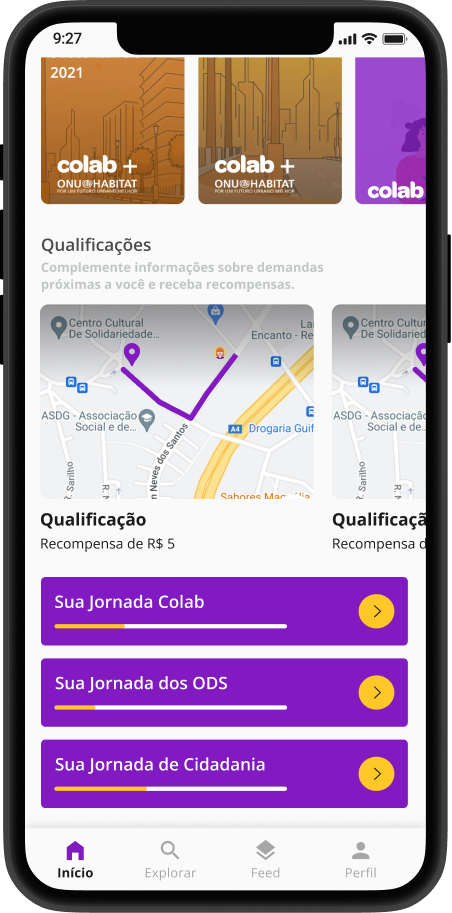
\includegraphics[width=0.33\textwidth]{images/colab_app_qualis.png}
\end{figure}

A gamificação no Colab não se limita apenas a incentivar a participação dos cidadãos. Ela também pode ser usada para conscientizar sobre determinadas causas ou estimular a participação em eventos. Por exemplo, se um hemocentro da cidade precisa de mais doações de sangue, a gestão pública pode criar um desafio no Colab para incentivar os cidadãos a doar sangue. Ao fazer isso, os cidadãos podem ganhar conquistas como "doador" ou "zelador do patrimônio público", reforçando a importância de suas contribuições para a cidade.

Em resumo, o Colab é uma plataforma que combina elementos de vigilância participativa, democracia digital e governo eletrônico para promover a participação cidadã na gestão pública. Através de suas diversas funcionalidades, o Colab busca fortalecer a participação cidadã, criar um ambiente propício para o diálogo entre cidadãos e governos, e promover a transparência e a responsabilidade no governo.

\section{e-Government e \textit{GovTechs}}

As \textit{GovTechs} são empresas que fornecem soluções tecnológicas para o setor público. Elas desempenham um papel crucial na modernização dos serviços governamentais, melhorando a eficiência, a transparência e a participação cidadã \cite{2022_Kononenko}. Os serviços prestados ao governo por empresas de \textit{GovTech} podem variar amplamente, dependendo das necessidades específicas do governo. Alguns exemplos incluem:

\begin{itemize}
	\item Digitalização de processos burocráticos: Isso pode incluir a criação de sistemas de gerenciamento de documentos, plataformas de pagamento online e sistemas de agendamento de compromissos. Por exemplo, muitas cidades adotam o Colab para integrar o processo de pagamento de impostos e taxas como o IPTU.
	\item Plataformas de participação cidadã: Estas são plataformas que permitem aos cidadãos participar diretamente na tomada de decisões do governo. Isso pode incluir a votação em questões políticas, a apresentação de propostas de políticas e a participação em discussões públicas.
	\item Soluções de análise de dados: As empresas de gov-tech podem fornecer soluções que ajudam o governo a coletar, analisar e interpretar grandes quantidades de dados. Isso pode ajudar o governo a tomar decisões mais informadas e eficazes.
\end{itemize}

O Colab é um exemplo de uma solução de \textit{GovTech} que se destaca na indústria pelo seu aspecto social. Como uma plataforma de participação cidadã, o Colab permite que os cidadãos se envolvam diretamente na tomada de decisões do governo, promovendo a transparência e a responsabilidade. Isso representa uma mudança significativa na forma como o governo interage com os cidadãos, permitindo uma maior inclusão e participação na tomada de decisões.

No entanto, a adoção de soluções de \textit{GovTech} como o Colab não está isenta de desafios. De acordo com um estudo de \citeonline{2021_Liang}, fatores como a competência do provedor, a prontidão organizacional, a pressão externa e a confiança na tecnologia desempenham um papel significativo na adoção de tecnologias de nuvem móvel no governo. Esses fatores podem ser igualmente aplicáveis ao Colab e outras soluções de \textit{GovTech}, e precisam ser considerados cuidadosamente ao implementar essas tecnologias.

\section{Interfaces para problemas urbanos}

No século XXI, a revolução digital desencadeou uma série de inovações, transformando as áreas urbanas em laboratórios de experimentação para soluções tecnológicas. Com o rápido crescimento da urbanização global e o surgimento de megacidades, a adoção de tecnologias como \sigla{IoT}{Internet das Coisas, a rede de dispositivos físicos conectados à internet, permitindo interação e coleta de dados.} e \sigla{IA}{Inteligência Artificial, o campo da ciência da computação dedicado a criar sistemas capazes de realizar tarefas que normalmente exigiriam inteligência humana.} tornou-se imperativa. As cidades inteligentes começaram a integrar sistemas digitais em suas operações diárias, buscando melhorar a qualidade de vida dos cidadãos.

Além do Colab, várias outras soluções surgiram globalmente para enfrentar os desafios urbanos. Em Barcelona, o projeto "Sentilo" utiliza sensores para monitorar tudo, desde a qualidade do ar até o nível de reservatórios \cite{2016_Sinaee_IP}. Em Cingapura, a iniciativa "Smart Nation" visa integrar a tecnologia digital em diversos aspectos da vida urbana \cite{2016_Chia_IP}.

Apesar do potencial evidente dessas interfaces digitais, elas também enfrentam críticas legítimas. Preocupações com a privacidade dos dados dos cidadãos, o potencial uso indevido das informações coletadas e a exclusão digital de segmentos da população são questões em debate. Além disso, a dependência excessiva da tecnologia pode reduzir a interação humana no processo de tomada de decisão.

No horizonte, a combinação de realidade aumentada, inteligência artificial e big data pode levar a soluções ainda mais avançadas. Imagine um mundo em que os cidadãos possam visualizar em tempo real os impactos de suas sugestões urbanas ou que os governos possam prever e mitigar problemas urbanos antes mesmo de ocorrerem, graças à análise preditiva.

É neste contexto de evolução urbana e tecnológica que o Colab se destaca como uma interface poderosa para a resolução de problemas urbanos. Além de facilitar a comunicação entre cidadãos e órgãos governamentais, o Colab reimagina a participação cidadã, tornando-a mais direta, transparente e democrática. O que o diferencia é a capacidade de promover a participação ativa e informada dos cidadãos, contrabalançando os efeitos negativos das câmaras de eco digitais.

Para ilustrar como o Colab tem sido eficaz nesse papel, vale a pena mencionar a pesquisa conduzida por \citeonline{2021_Barros} em que o Colab foi avaliado juntamente com outras duas iniciativas de democracia digital, Mudamos e Panela de Pressão. A avaliação considerou diferentes aspectos, como recursos tecnológicos, modos de participação online, atores envolvidos, objetivos políticos das iniciativas e captação de recursos. Os resultados destacaram a importância da estrutura organizacional na compreensão do desenvolvimento bem-sucedido de iniciativas de democracia digital.

\citeonline{2015_Silva} analisaram o Colab como uma ferramenta de colaboração e mobilidade urbana. Esse estudo ressaltou a relevância do Colab como uma plataforma que permite aos cidadãos participarem ativamente da melhoria de suas cidades, fornecendo um canal direto de feedback às autoridades municipais sobre problemas urbanos.

O estudo de \citeonline{2018_CARVALHO_DISSERTATION} explora o uso do Colab para promover a participação social na gestão da cidade de Paragominas, no estado do Pará, Brasil. Apesar de Paragominas ser uma cidade relativamente isolada, o estudo demonstrou que a implementação do Colab resultou em um canal eficaz de comunicação entre a prefeitura e os cidadãos, alcançando o maior percentual de usuários do aplicativo em todo o estado do Pará. As conclusões de Carvalho indicam que a Computação Urbana e o uso de dispositivos móveis podem fortalecer as relações entre os usuários e ajudar a entender melhor como os problemas pontuais afetam a cidade como um todo. O estudo destaca o potencial da Computação Urbana e de aplicativos móveis para melhorar a gestão das cidades, promovendo a participação social e melhorando a comunicação entre os cidadãos e as autoridades municipais, mesmo em áreas isoladas como Paragominas.

A pesquisa realizada por \citeonline{2020_Seno_PHD} na cidade de Santo André, São Paulo, oferece uma perspectiva aprofundada sobre a implementação e impacto do Colab em um contexto municipal. Este estudo meticuloso analisou como a plataforma Colab foi adotada pela administração municipal entre 2017 e 2020, destacando o papel crucial das capacidades tecnológicas na gestão de serviços urbanos. Através de entrevistas com atores-chave e observação participante, o estudo de Seno revelou que a implementação do Colab exigiu não apenas a mobilização de recursos tecnológicos e infraestrutura, mas também uma coordenação eficaz entre diferentes áreas e atores governamentais. Os resultados apontaram para um aumento significativo na eficiência da gestão de dados e informações, contribuindo para uma prestação de serviços mais ágil e responsiva. Este caso de Santo André ilustra como plataformas como o Colab podem transformar a interação entre cidadãos e governo, promovendo uma participação mais ativa e informada na gestão urbana, alinhando-se assim com as tendências emergentes de cidades inteligentes e participativas.

Esses estudos de caso fornecem evidências concretas de como o Colab tem sido uma interface valiosa na resolução de problemas urbanos. Sua capacidade de promover a participação cidadã, coletar feedback dos cidadãos e melhorar a prestação de serviços públicos o torna uma ferramenta relevante para impulsionar mudanças positivas nas cidades. Através do Colab e de outras interfaces similares, é possível fortalecer a colaboração entre os cidadãos, autoridades municipais e outros atores envolvidos na busca por soluções inovadoras e sustentáveis para os desafios urbanos. Essas plataformas estão pavimentando o caminho para um futuro urbano mais inteligente e participativo.

\section{Vigilância Participativa na Era da COVID-19}

A pandemia de COVID-19 apresentou desafios sem precedentes para a participação cidadã e o engajamento social. Em resposta a esses desafios, plataformas digitais emergiram como ferramentas vitais para facilitar a participação cidadã na gestão pública, mesmo em meio ao distanciamento social. Este cenário acelerou a adoção de tecnologias que permitem o envolvimento direto dos cidadãos em processos de vigilância e monitoramento.

\subsection*{Vigilância Participativa}
A vigilância participativa é uma abordagem inovadora que envolve o engajamento ativo da comunidade no processo de coleta, monitoramento e compartilhamento de informações relevantes para identificar e responder a problemas sociais, ambientais e de saúde.

\begin{citacao}
\textit{“…uma forma de inteligência coletiva em que as pessoas se reúnem para monitorar, analisar e agir coletivamente em relação a um problema ou questão compartilhada.”}
\fdireta{2011_Bryer}
\end{citacao}

Com os avanços tecnológicos e a disseminação de dispositivos móveis e plataformas digitais, a aplicação de aplicativos móveis para a vigilância participativa tem ganhado destaque. Nesta seção, exploramos o conceito de vigilância participativa, apresentando sua definição e abordando sua relevância no contexto atual.

A vigilância participativa tem sido reconhecida como uma abordagem promissora para a coleta de informações em tempo real, permitindo que a comunidade desempenhe um papel ativo na detecção e monitoramento de problemas sociais, ambientais e de saúde. Tradicionalmente, a vigilância tem sido realizada por meio de sistemas centralizados e conduzida por especialistas em saúde ou autoridades governamentais. No entanto, com a proliferação de dispositivos móveis, o acesso à internet e o surgimento de plataformas colaborativas, os aplicativos móveis têm sido adotados como ferramentas eficazes para engajar os cidadãos na vigilância participativa.

O conceito de vigilância participativa foi formalmente reconhecido pelas Regulamentações Sanitárias Internacionais (RSIs) revisadas em 2005, as quais ampliaram o escopo da vigilância além dos mecanismos tradicionais. Esse reconhecimento proporcionou uma oportunidade para a integração de canais não oficiais e melhorias tecnológicas para agilizar a detecção, o monitoramento e a resposta a problemas de saúde. A vigilância participativa utiliza métodos de crowdsourcing para coletar informações da sociedade e devolver o conhecimento coletivo de volta à comunidade \cite[1]{2017_Smolinski}.

\subsubsection*{Estudo de Caso: Saúde na Copa}
Um estudo de caso relevante que exemplifica a aplicação da vigilância participativa é a iniciativa "Saúde na Copa" durante a Copa do Mundo FIFA de 2014, realizada no Brasil. O projeto utilizou um aplicativo de vigilância participativa chamado Healthy Cup, permitindo que usuários de todo o mundo relatassem suas condições de saúde em tempo real. Ao focar em três síndromes específicas e seis doenças relevantes para aglomerações de pessoas, o aplicativo facilitou a detecção precoce de surtos de doenças agudas ao identificar agregados de sintomas indicativos de doenças infecciosas \cite{2017_LealNeto}.

Além da saúde, a vigilância participativa também tem sido aplicada em outras áreas, proporcionando benefícios semelhantes e promovendo a participação ativa da comunidade. Essa abordagem colaborativa tem se mostrado útil na vigilância de diversos aspectos do ambiente e da sociedade, permitindo que os cidadãos desempenhem um papel ativo na coleta e compartilhamento de informações relevantes.

\subsubsection*{Monitorização do Ruído Ambiental}
Outra área em que a vigilância participativa tem desempenhado um papel importante é a monitorização do ruído ambiental. O aplicativo NoiseTube permite que os usuários realizem medições de ruído e compartilhem esses dados, criando um mapa colaborativo do ruído em diferentes localidades. Essa vigilância participativa do ruído ambiental permite a identificação de áreas com altos níveis de ruído, auxiliando na tomada de medidas para mitigar os efeitos adversos na saúde e no bem-estar da comunidade. Ao participar ativamente da vigilância do ruído, os cidadãos contribuem para a criação de ambientes mais saudáveis e para a implementação de políticas públicas adequadas \cite{2010_Arnand}.

\begin{figure}[!htb]
	\caption{Aplicativo NoiseTube exibindo o nível de ruído em uma localidade}
	\label{fig
	}
	\centering
	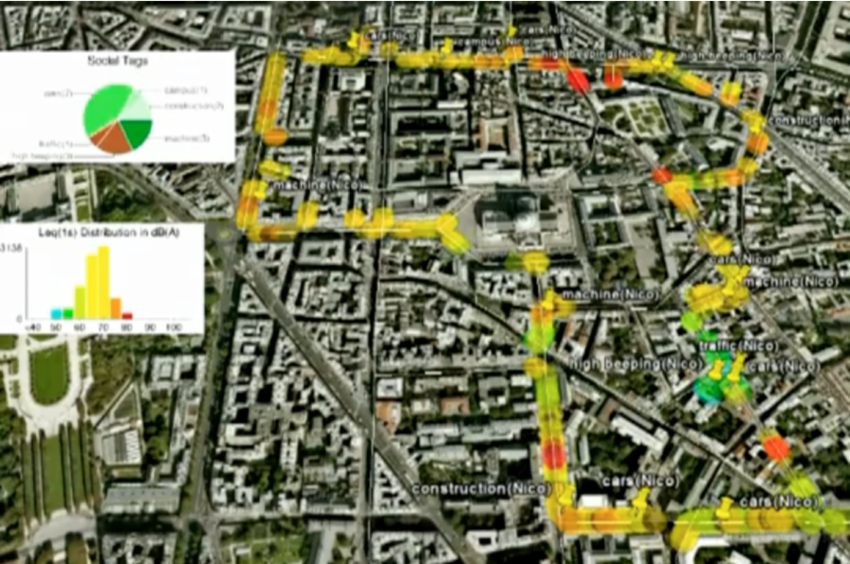
\includegraphics[scale=0.8]{app_noisetube.png}
	\fdireta{2010_Arnand}
	\end{figure}

Esses exemplos ilustram como a vigilância participativa pode ser aplicada em diferentes áreas, além da saúde. Ao envolver os cidadãos na coleta e compartilhamento de informações relevantes, a vigilância participativa se torna uma ferramenta poderosa para a identificação e resposta a problemas ambientais e sociais. Essa abordagem colaborativa, combinada com o uso de tecnologias móveis e plataformas digitais, fortalece a relação entre a comunidade e as autoridades responsáveis, promovendo uma governança mais inclusiva e eficaz.

\subsection*{Iniciativa Brasil Sem Corona}
A Iniciativa Brasil Sem Corona, uma colaboração entre o Colab e a startup Epitrack, exemplifica o uso eficaz da tecnologia para facilitar a participação cidadã durante uma crise de saúde pública. Através desta iniciativa, os dados sobre a pandemia de COVID-19 foram coletados diretamente dos cidadãos, que relataram seus sintomas e receberam informações sobre como se proteger do vírus. Esses dados foram então utilizados para gerar mapas de calor que auxiliaram as autoridades de saúde a identificar e responder a surtos de COVID-19.

Na cidade de Caruaru/PE, a iniciativa teve resultados significativos. O projeto contou com 861 usuários ativos, apresentando uma média de 1,2 relatórios por usuário por semana. A plataforma Brasil Sem Corona começou em 20 de março e, desde então, tem sido oficialmente utilizada pela autoridade de saúde de Caruaru para melhorar a qualidade das informações do sistema de vigilância tradicional. Em relação aos casos de síndrome respiratória do sistema de vigilância tradicional, 1.588 indivíduos foram positivos para este resultado clínico. A análise de varredura espacial detectou 18 aglomerados e 6 deles apresentaram significância estatística (valor p < 0,1). Os aglomerados 3 e 4 apresentaram uma área de sobreposição que foi escolhida pela autoridade local para implantar a sorologia de Covid-19, onde 50 indivíduos foram testados. Desses, 32\% (n=16) apresentaram resultados reagentes para anticorpos relacionados à Covid-19 \cite[1]{2020_LealNeto}. Essa pesquisa demonstra como a vigilância participativa pode ser uma ferramenta eficaz para melhorar a qualidade das informações do sistema de vigilância tradicional, permitindo uma detecção precoce de surtos de COVID-19 e uma resposta mais eficaz, principalmente quando aliado a uma aplicação de alta disponibilidade e adoção pela população.

\subsection*{Conclusão}
Os exemplos apresentados ilustram a viabilidade e a utilidade da vigilância participativa como uma abordagem para a gestão de crises e problemas sociais. O Colab, como uma rede social de cidadania, diferencia-se de outras plataformas, como o Twitter, onde o comportamento tende a ser mais combativo e centrado em reclamações. No Colab, os usuários estão naturalmente mais inclinados a participar de forma colaborativa, o que torna a plataforma especialmente adequada para campanhas de vigilância participativa.

Essa predisposição dos usuários para contribuir positivamente cria uma vasta malha de dados que pode ser analisada para obter insights valiosos. Do ponto de vista de dados e engenharia de software, essa riqueza de informações permite entender melhor o comportamento dos usuários e identificar os fatores que incentivam a participação na vigilância participativa. Além disso, essa análise pode ajudar a diferenciar entre contribuições positivas e negativas, evitando a formação de câmaras de eco e promovendo um ambiente mais saudável para a colaboração cidadã.

Portanto, o Colab não só valida a eficácia da vigilância participativa, mas também demonstra como plataformas digitais podem ser utilizadas para promover uma governança mais inclusiva e participativa, incentivando os cidadãos a desempenharem um papel ativo na melhoria da sociedade. No entanto, à medida que a sociedade digitaliza os seus problemas reais, é crucial refletir sobre como esses eventos ou fenômenos da realidade são representados no mundo digital. A hiper-realidade, um conceito filosófico introduzido por Jean Baudrillard, pode fornecer uma lente valiosa para entender essa dinâmica, iluminando como a interação entre cidadãos e governos se transforma nesse espaço digital.

\section{Gov-Techs, Participação Cidadã e Hiper-realidade}

\begin{citacao}
	\small{
		\textbf{Do rigor da ciência}

		\textit{“…Naquele  Império,  a  Arte  da  Cartografia  alcançou  tal  perfeição  que  o  mapa  de  uma  única  Província  ocupava  toda  uma  Cidade,  e  o  mapa  do  Império,  toda  uma  Província. Com o tempo, esses Mapas Desmedidos não foram satisfatórios e os Colégios de Cartógrafos levantaram um Mapa do Império, que tinha o tamanho do Império e coincidia pontualmente com ele. Menos afeiçoadas ao Estudo da  Cartografia,  as  Gerações  Seguintes  entenderam  que  esse dilatado Mapa era Inútil e não sem Impiedade o entregaram às Inclemências do Sol e dos Invernos. Nos desertos do Oeste perduram despedaçadas Ruínas do Mapa, habitadas por Animais e por Mendigos; em todo o País não há  outra  relíquia  das  Disciplinas  Cartográficas.”}

		\textit{Jorge Luis Borges}
	}
	\fdireta{2012_Melendi}
\end{citacao}

\begin{figure}[!htb]
	\centering
	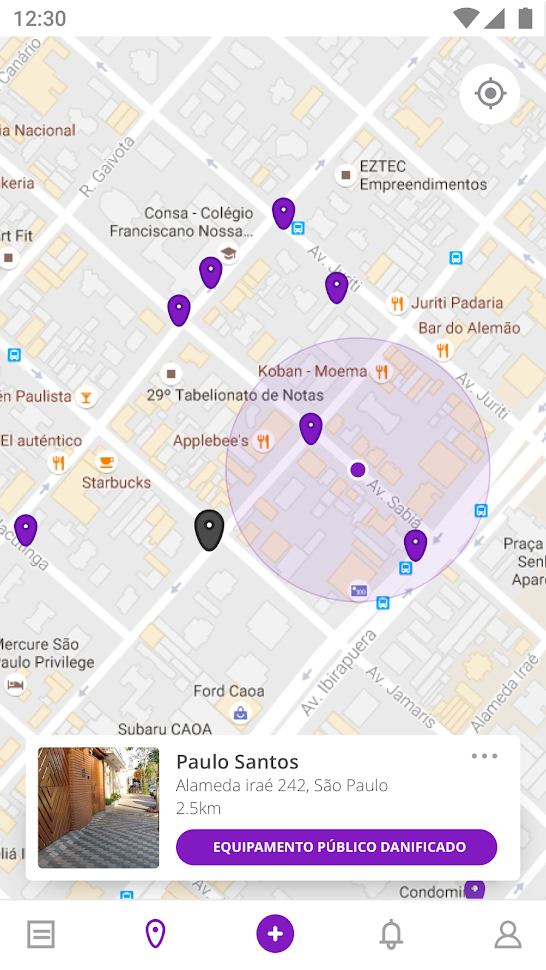
\includegraphics[width=0.48\textwidth]{images/colab_app_map.png}
	\caption{Mapa de eventos reportados no Colab}
	\label{fig:colab_app_map}
\end{figure}

O surgimento das Gov-Techs, empresas especializadas em atender demandas governamentais, e a identificação do Colab como uma rede social de participação cidadã representam um avanço notável na interação entre cidadãos e governos. No mundo real, essa relação entre governo e cidadão e seus papéis e responsabilidades são geralmente demarcados por estruturas burocráticas e um conjunto de protocolos formais.

Essa dinâmica tradicional é desafiada no ambiente digital, onde as relações assumem uma forma mais fluida e interativa. Após realizarmos uma análise superficial de algumas postagens no Colab, percebemos que a hiper-realidade oferece uma perspectiva valiosa para entender essas novas dinâmicas digitais, iluminando como a interação entre cidadãos e governos se transforma nesse espaço. Essa perspectiva não apenas lançou luz sobre alguns fenômenos iniciais observados, mas também informou diretamente nossas decisões de desenvolvimento de software e interpretações derivadas dos dados da plataforma, emprestando uma forma de olhar questões de participação cidadã e governança. Neste tópico, detalharemos alguns desses fenômenos e como a perspectiva da hiper-realidade nos ajudou a interpretá-los.

A hiper-realidade, um conceito amplamente discutido por Jean Baudrillard, descreve uma condição na qual a realidade se dissolve em uma simulação tão convincente que a distinção entre o real e o imaginário se torna sutil e evasiva. Baudrillard introduz o conceito de 'simulacro' para descrever essa simulação, que não é apenas uma cópia da realidade, mas uma representação que se torna realidade em si \cite{1994_Baudrillard_BOOK}. No contexto do Colab, essa dinâmica se manifesta quando os eventos reportados na plataforma, embora sejam reflexos de problemas urbanos reais, podem ser interpretados como realidades independentes. Estes 'simulacros' de problemas urbanos, amplificados pela interatividade e engajamento digital, podem às vezes obscurecer a realidade física subjacente, criando um espaço onde a dimensão digital influencia diretamente a resposta governamental e a percepção pública do problema.

Cada evento reportado no aplicativo, portanto, não é apenas uma demanda real da cidade, mas também a representação dessa demanda dentro de um ambiente digital: um hipertexto; multimídia, geolocalizado, verificável. Os dados do Colab, portanto, representam cartograficamente a cidade de uma forma que ecoa a ideia de Borges sobre a sobreposição do mapa e do território. Tal como no poema, em que o mapa se torna tão abrangente e detalhado que se confunde com o próprio território que representa, os eventos reportados no Colab criam um 'mapa digital' que, em muitos aspectos, começa a se assemelhar e até mesmo substituir a experiência do espaço urbano real. Esta sobreposição entre a realidade física e sua representação digital ilustra vividamente a noção de simulacro de Baudrillard: o mapa digital no Colab não é apenas um reflexo da cidade, mas uma recriação dela que ganha sua própria realidade e influência.

O usuário, ao postar sobre um problema, atua como um avatar de um cidadão, criando uma camada de representação que pode ou não corresponder fielmente à realidade. Esta dualidade entre o evento real e sua representação digital é um exemplo clássico da hiper-realidade. Por exemplo, ao reportar eventos de zeladoria pública, o usuário pode escolher um tipo de evento pré-definido. Apesar de existirem dezenas de tipos de eventos, muitos usuários reportam eventos em categorias errôneas, de forma não deliberada. Isso ocorre quando a representação digital do evento se desvia da realidade, já que a categorização inadequada pode distorcer a percepção pública e governamental do problema, ou o usuário pode não ter encontrado a categoria de evento mais apropriada. Além disso, em algumas situações, eventos são postados em categorias que geram mais engajamento, visando obter mais visibilidade, mesmo que o evento não tenha uma relação direta com a categoria original. Esses fenômenos podem causar subnotificação de algumas categorias e supernotificação equivocada em outras categorias de eventos.

Outro aspecto de hiper-realidade pode ser observado nas cópias de eventos para o mesmo problema reportado por diferentes usuários. Cada um com uma descrição subjetiva do problema. Por exemplo, situações relacionadas ao esgoto e saneamento básico podem apelar para o sentimento de meio ambiente e saúde pública em alguns usuários, enquanto a outros podem evocar sentimentos de limpeza e ordem. Isso resulta em várias representações digitais do mesmo problema, cada uma moldada pelas perspectivas individuais dos usuários. Essas simulacros podem ser mais ou menos precisos em relação à realidade física, mas, em última análise, são versões da realidade que existem independentemente da demanda concreta.

\begin{figure}[!htb]
	\centering
	\begin{subfigure}{0.4\textwidth}
		\centering
		
\includegraphics[width=\linewidth]{images/colab_hiper_reality_corr_01.png}
		\caption{Postagem no Twitter}
		\label{fig:colab_hiper_reality_corr_01}
	\end{subfigure}
	\hspace{5mm}
	\begin{subfigure}{0.6\textwidth}
		\centering
		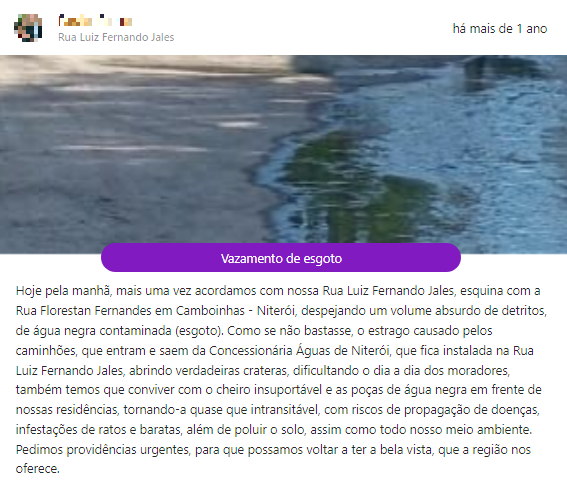
\includegraphics[width=\linewidth]{images/colab_hiper_reality_corr_02.PNG}
		\caption{Postagem original no Colab}
		\label{fig:colab_hiper_reality_corr_02}
	\end{subfigure}
	\caption{Exemplo de correlação entre evento reportado no Colab e replicado no Twitter}
	\label{fig:colab_hiper_reality}
\end{figure}

OOutro fenômeno intrigante que emerge na interseção da hiper-realidade e da participação cidadã é a tendência dos usuários em replicar eventos do Colab em outras plataformas, como ReclameAqui e Twitter. Esta ação reflete um aspecto fundamental da hiper-realidade: a disseminação de representações digitais que transcendem as fronteiras da plataforma original. Nesse contexto, cada evento reportado no Colab não é apenas uma demanda específica da cidade, mas também uma representação digital dessa demanda que adquire vida própria. Quando um usuário replica um evento em outra rede social, ele está, de fato, criando um simulacro do problema urbano. Esses simulacros, embora compartilhem uma raiz comum na demanda original, são moldados pelas perspectivas individuais dos usuários e pelas normas e convenções das plataformas em que são postados.

O impacto desse fenômeno é profundo. Cada replicação estende ainda mais a camada de hiper-realidade, multiplicando as representações digitais de um único problema. Essas cópias não apenas adicionam complexidade à percepção do problema, mas também desafiam a noção tradicional de uma realidade única e objetiva. A hiper-realidade nos ensina que a realidade física e sua representação digital são intrinsecamente entrelaçadas, e as cópias de eventos demonstram essa interconexão de maneira vívida. No entanto, também é importante reconhecer que, à medida que essas representações digitais se multiplicam, há um risco de que a substância do problema original se perca em meio à diversidade de perspectivas e interpretações.

A busca pela autenticidade na resolução de demandas urbanas pode ser obscurecida pela multiplicidade de representações, cada uma com sua própria ênfase e contexto. Além disso, o poder de amplificação das redes sociais como o Twitter pode transformar uma representação digital em uma narrativa amplamente reconhecida ou distorcê-la completamente, influenciando a percepção pública e governamental do problema. Portanto, à medida que exploramos a hiper-realidade, é crucial considerar como essas cópias de eventos afetam a dinâmica da participação cidadã e a resposta governamental, bem como o papel das redes sociais na amplificação dessas representações digitais.

Voltando ao Colab, vale mencionar que a seleção de imagens e mídia associada a um evento pode moldar significativamente sua representação. Por exemplo, a escolha de uma foto de um parque coberto de lixo em um relato de zeladoria pública pode evocar uma resposta emocional mais forte em comparação com uma imagem mais neutra. Isso ilustra como a hiper-realidade também se estende à seleção e apresentação de mídia, influenciando a percepção do problema e suas possíveis soluções.

Além disso, eventos aparentemente simples podem desencadear debates complexos e amplificados na plataforma. Por exemplo, um relato sobre um buraco na estrada pode se transformar em uma discussão sobre o estado geral da infraestrutura da cidade, com diversos usuários adicionando suas próprias camadas de interpretação e significado ao evento inicial. Essa expansão da discussão em torno de um evento simples é outra manifestação da hiper-realidade, onde a materialidade se transmuta em múltiplas representações digitais, cada uma com suas próprias nuances e subjetividades. Esses debates, por vezes, resultam na formação de "câmaras de eco" dentro da plataforma, em que grupos de usuários compartilham perspectivas semelhantes, reforçando ainda mais suas crenças e opiniões, muitas vezes isolando-se de visões divergentes. Isso ilustra como a hiper-realidade também pode contribuir para a polarização das discussões e a formação de bolhas de percepção, onde as múltiplas representações digitais da realidade podem não apenas coexistir, mas também se separar em compartimentos isolados, tornando ainda mais complexa a busca pela compreensão e solução de problemas urbanos.

No \autoref{chapter:08_hyperlocalbarometer}, exploramos mais profundamente como a hiper-realidade pode criar ambientes com pressão social hiperlocalizada, em que certas comunidades de usuários tendem a priorizar demandas urbanas específicas e não se engajam com os problemas urbanos como um todo. Por exemplo, usuários que reportam problemas de trânsito tendem a não reportar problemas de mobilidade urbana e vice-versa. Apesar de conviverem no mesmo espaço físico, as demandas digitais mostram dois mundos paralelos. O que acontece quando essas duas hiper-realidades colidem?

Revisitar o poema de Borges, sob a perspectiva da hiper-realidade, nos oferece inicialmente uma crítica da cartografia digital: a representação, por mais detalhada que seja, perde seu valor se não conduzir à ação e à mudança na realidade que ela busca mapear. No contexto do Colab, esta lição é vital. O objetivo não se limita a criar um mapa digital detalhado e informativo, ocupando \textit{buckets} de armazenamento em uma nuvem de dados.

O poema também é uma chamada para ação: o cerne está em usar essa representação digital como uma alavanca para ações efetivas na paisagem urbana. A cartografia de demandas no Colab não é apenas um exercício de documentação, mas um instrumento para identificar e responder às necessidades urbanas. Ao propor heurísticas de detecção de câmaras de eco, que são o foco deste estudo, buscamos reconfigurar a maneira como interagimos com os dados existentes, propondo um dinamismo renovado, prevenindo a estagnação de informações e incentivando a transformação contínua do nosso ambiente urbano. Dessa forma, o Colab transcende a armadilha do 'Mapa Desmedido' de Borges, empregando a representação digital não como um fim, mas como um meio dinâmico de interpretar a hiper-realidade para a melhoria contínua do tecido urbano.

\subsection*{Críticas à Hiper-realidade}

Além de Baudrillard, outros autores também exploraram conceitos semelhantes. Umberto Eco, em sua obra "Viagem na Irrealidade Cotidiana", discute como a cultura popular e os meios de comunicação criam versões da realidade que, muitas vezes, são mais atraentes do que a própria realidade \cite{1993_Eco_BOOK}. Guy Debord, com a teoria da "Sociedade do Espetáculo", argumenta que a vida moderna se tornou uma série de representações, onde a imagem tem mais valor do que a experiência direta \cite{1993_Eco_BOOK}. Ao refletir sobre as interações no Colab à luz da hiper-realidade, percebemos que a plataforma não apenas aprimora a comunicação entre cidadãos e governos, mas também cria um ambiente em que a realidade urbana é continuamente reconstruída e reinterpretada digitalmente. Essa reinterpretação constante nos leva a questionar a autenticidade e a precisão das representações dos problemas urbanos na plataforma. Enquanto as ideias de Heidegger e Merleau-Ponty sobre inautenticidade oferecem insights valiosos, é importante reconhecer que, em um mundo pós-moderno, a noção de autenticidade pode ser altamente relativa e influenciada pelo contexto cultural e social.

A concepção de Heidegger sobre inautenticidade, centrada na perda de uma conexão genuína com o mundo e na adoção de representações superficiais, oferece uma perspectiva importante, mas que necessita de recontextualização no cenário da pós-modernidade e da hiper-realidade digital. 

No ambiente digital, particularmente em plataformas como o Colab, a noção de autenticidade enfrenta novos desafios. Em uma era definida pela multiplicidade de realidades e perspectivas, a autenticidade não é mais uma questão de aderência a uma experiência ou realidade 'verdadeira' e unidimensional. Ao contrário, no ciberespaço, a experiência autêntica é frequentemente dinâmica, refletindo uma variedade de verdades e realidades que coexistem e se sobrepõem. Por exemplo, no Facebook, uma pessoa pode compartilhar momentos pessoais e informais, enquanto no LinkedIn, a mesma pessoa apresenta uma versão mais profissional e formal de si mesma. No Colab, um usuário pode assumir o papel de um cidadão engajado e preocupado com questões urbanas, o que pode ser diferente de como ele se apresenta em outras redes sociais. Essa variação não significa necessariamente inautenticidade no sentido tradicional que Heidegger propôs. Em vez disso, reflete a complexidade da identidade humana na era digital, um espaço onde múltiplas "autenticidades" podem coexistir. Cada uma dessas representações é autêntica em seu próprio contexto e serve a diferentes propósitos e aspectos da vida de uma pessoa.

É importante reconhecer, no entanto, que muitos comportamentos nas redes sociais não emergem organicamente, mas são engenhosamente projetados pelas próprias plataformas. Estes ambientes digitais frequentemente incentivam a formação de relacionamentos parassociais, em que os usuários desenvolvem conexões unilaterais com figuras públicas ou entidades representadas digitalmente. Esta dinâmica engendrada pode complicar ainda mais as noções de autenticidade e inautenticidade. Em vez de uma simples desconexão com a realidade, como sugerido por Heidegger, a inautenticidade no contexto digital pode ser uma consequência da interação com sistemas projetados para moldar comportamentos e percepções. Isso desafia a abordagem binária de Heidegger, sugerindo que a autenticidade digital pode ser encontrada na capacidade de navegar e dar sentido a essas múltiplas realidades, e na conscientização de como as estruturas e algoritmos das plataformas digitais influenciam essas interações, em vez de aderir a uma noção singular e imutável de verdade.

Merleau-Ponty destaca a importância da percepção autêntica do mundo, que envolve uma relação direta e imediata com nosso ambiente. No entanto, em um ambiente digital como o Colab, essa relação direta é frequentemente mediada por interfaces e representações digitais. Isso levanta a questão de se a percepção autêntica ainda é possível em um contexto digital onde as experiências são filtradas por dispositivos e plataformas. Portanto, é crucial considerar como a hiper-realidade afeta não apenas a comunicação, mas também a construção da autenticidade da participação cidadã e da percepção dos problemas urbanos. Nesse sentido, é importante reconhecer que o conceito de autenticidade pode ser altamente variável e influenciado pelo contexto, desafiando as definições tradicionais de Heidegger e Merleau-Ponty no mundo do ciberespaço.

Críticos contemporâneos de Baudrillard, como Douglas Kellner, oferecem uma perspectiva crítica sobre a hiper-realidade, enfatizando como ela pode conduzir a uma despolitização e passividade na sociedade. Kellner alerta que, em um mundo dominado por imagens e simulações, existe o risco de que estas substituam a ação e o engajamento real \cite{1995_Kellner_BOOK}. No contexto de plataformas como o Colab, essa crítica adquire uma dimensão adicional. Embora o Colab incentive a participação cidadã através de mecanismos de gamificação e aspectos sociais, levanta-se a questão sobre a profundidade e autenticidade desse engajamento. Os usuários são motivados a reportar problemas urbanos não por recompensas materiais, mas por uma satisfação psicológica e social derivada do reconhecimento e pertencimento dentro da comunidade virtual.

Uma leitura dessa interpretação de Kellner pode sugerir que, enquanto essas plataformas podem parecer aumentar a participação cidadã, elas também podem criar uma camada de simulação que obscurece a distinção entre engajamento cívico genuíno e atividades motivadas por recompensas simbólicas. Essa análise nos desafia a considerar se as ações no Colab representam uma verdadeira mudança cívica ou se são meramente expressões de uma realidade hiper-real, em que a imagem do engajamento substitui a substância do mesmo.

No entanto, ao interpretar os dados do Colab sob a perspectiva da hiper-realidade, podemos analisar problemas de dados sob um novo prisma focado principalmente em como as representações digitais influenciam a percepção e a resolução de problemas urbanos. Por exemplo, ao criar Personas que representam diferentes tipos de usuários com motivações e padrões de postagens distintos, podemos explorar como a hiper-realidade molda as interações e expectativas dentro da plataforma. 

As Personas podem servir como lentes valiosas para compreender como as representações digitais afetam a percepção pública e governamental dos problemas urbanos, oferecendo uma visão mais profunda das complexas dinâmicas que permeiam o Colab. Além disso, cabe analisar como a hiper-realidade afeta a percepção e a resposta governamental aos problemas urbanos. 

Analisar como eventos são categorizados e priorizados, por exemplo, pode revelar como a hiper-realidade influencia a alocação de recursos e esforços. Essas análises podem fornecer insights valiosos sobre como a hiper-realidade afeta a participação cidadã e a governança, permitindo que os governos e cidadãos compreendam melhor as complexas dinâmicas que permeiam a plataforma. No próximo tópico, exploraremos como a hiper-realidade pode influenciar a percepção e a resposta governamental aos problemas urbanos.

\subsection*{Desafios da Hiper-realidade na Resolução de Demandas Urbanas}

No contexto mais amplo, considerando os serviços prestados pelo Colab como \textit{Gov-Tech}, a utilização de dados de eventos de zeladoria pública por agências governamentais para estabelecer \textit{pipelines} de resolução de demandas na cidade representa um fenômeno intrigante no âmbito da hiper-realidade. Um exemplo notável dessa abordagem pode ser observado em Mesquita, no Rio de Janeiro, onde a taxa de resolução de demandas atingiu impressionantes 95\% em 2021 \cite{2021_Colab_PAGE}. Através do Colab, a prefeitura implementou um sistema de gestão estratégica que integra o feedback dos cidadãos diretamente em suas operações. Ramon Lameira, gerente de Implementação e Operações do Colab na Secretaria de Planejamento da Prefeitura, descreve essa abordagem da seguinte maneira:

\begin{citacao}
\textit{“…O setor de planejamento estratégico na prefeitura tem no Colab uma ferramenta importante na cidade, a gente tem um tripé de governo muito baseado em demandas do cidadão pelo Colab. (Tem um) núcleo de dados, então a gente faz toda a coleta de indicadores e a coleta de serviços, e uma equipe de projetos estratégicos na prefeitura, então a gente junta essas três áreas para poder executar todos os projetos da cidade.”}
\fdireta{2021_Colab_PAGE}
\end{citacao}

Nesse cenário, é notável que as autoridades municipais frequentemente tomam conhecimento de questões urbanas através dos relatos dos usuários na plataforma. No entanto, é importante reconhecer que essa dinâmica de comunicação não é acessível para todos os cidadãos, uma vez que nem todos têm acesso ao aplicativo ou a habilidade de utilizá-lo, o que levanta questões de inclusão. Aqueles que têm acesso a dispositivos móveis e habilidades digitais são mais propensos a usar o Colab, enquanto cidadãos marginalizados, que muitas vezes enfrentam os problemas urbanos mais graves, podem ser deixados de fora da narrativa digital. Portanto, é importante lembrar que, embora o Colab ofereça uma plataforma valiosa para a participação cidadã, a realidade urbana é mais complexa e a representação digital nem sempre captura de forma equitativa todas as vozes e experiências.

Assim, a representação digital das demandas urbanas no Colab ganha uma importância que transcende a existência física da demanda em si. Problemas que não são relatados na plataforma podem permanecer invisíveis para as autoridades, mesmo que estejam presentes na realidade urbana. Essa dinâmica levanta uma questão crucial sobre a influência da hiper-realidade nesse processo. Além disso, a dinâmica de engajamento digital no Colab, como rede social de cidadania, pode influenciar a percepção das agências governamentais sobre a priorização das demandas. Eventos reportados por usuários com um número significativo de seguidores ou aqueles que geram maior interação na plataforma podem ser percebidos como mais urgentes ou relevantes. Isso pode, hipoteticamente, levar a uma distorção na alocação de recursos e esforços, em uma dinâmica onde a visibilidade digital, e não a gravidade real do problema, dita a priorização. No entanto, a abordagem estratégica de três fases adotada pela Prefeitura de Mesquita parece considerar a gravidade do problema além de sua visibilidade digital.

Outro aspecto da hiper-realidade se manifesta nas respostas automáticas fornecidas pelas agências governamentais. Frequentemente, essas respostas consistem em números de protocolo ou mensagens padronizadas, sem uma interação humana direta. Nossa análise inicial do sentimento das postagens no Colab revela que essa falta de interação personalizada pode gerar frustração entre os usuários. Eles se deparam com uma interface que, embora eficiente em catalogar e responder a problemas, falha em fornecer um sentido de engajamento humano genuíno. Essa dinâmica reflete uma característica central da hiper-realidade, onde a simulação de uma resposta (um número de protocolo ou uma mensagem automatizada) substitui a experiência de uma interação humana autêntica, reforçando a sensação de que, embora os problemas sejam reportados e reconhecidos, eles são tratados mais como dados em um sistema do que como questões que afetam a vida real das pessoas.

\subsection*{Desenvolvimento de Software e Fenomenologia na Era da Hiper-realidade}

Na análise do impacto do Colab na resolução de problemas urbanos, é essencial considerar a influência da hiper-realidade na percepção e resposta a esses problemas. A interação entre a realidade física dos problemas urbanos e sua representação no Colab gera uma camada complexa de realidade, onde a dimensão digital e a realidade física se entrelaçam, desafiando as abordagens tradicionais de governança e participação cidadã. Esta intersecção destaca a importância de uma abordagem fenomenológica, que enfatiza a percepção e experiência subjetiva dos indivíduos.

Ao adotar essa perspectiva, podemos compreender melhor como os usuários do Colab experienciam e interpretam a realidade urbana e sua representação digital, reconhecendo que essas percepções moldam a realidade vivida e, consequentemente, as respostas políticas e sociais. Por exemplo, ao considerar simulações, a Modelagem Baseada em Agentes (MBA) serve como um exemplo ilustrativo de como a perspectiva fenomenológica pode informar e enriquecer nossas heurísticas no campo da engenharia de software. Nessa perspectiva, os usuários do Colab podem ser modelados como agentes individuais, cada um com suas próprias percepções, motivações e comportamentos, destilando algumas dessas características em Personas. A MBA nos permite explorar como as interações entre esses agentes e o ambiente digital do Colab geram padrões emergentes de participação e resposta a problemas urbanos. Esta abordagem não é apenas uma ferramenta técnica; ela reflete um compromisso com a compreensão profunda das experiências subjetivas dos usuários. Essas dinâmicas são introduzidas em detalhes no \autoref{05_mba}.

Ao imaginar heurísticas de desenvolvimento de software sob essa perspectiva fenomenológica, reconhecemos que qualquer análise ou solução que ignore as dimensões subjetivas e experiências dos usuários é, em certo sentido, incompleta. A fenomenologia, portanto, não é apenas uma lente teórica, mas uma orientação prática essencial para o desenvolvimento de tecnologias digitais como o Colab. Ela nos lembra que, por trás de cada interação digital, há uma experiência humana rica e subjetiva. Isso é particularmente crucial sob a perspectiva da hiper-realidade, onde a distinção entre a representação digital e a experiência física se torna cada vez mais fluida. Uma abordagem fenomenológica assegura que as tecnologias que desenvolvemos sejam não apenas funcionalmente eficazes, mas também profundamente alinhadas com a complexidade da experiência humana em um mundo cada vez mais digitalizado.

Para enfrentar os desafios apresentados pela hiper-realidade, é crucial que os desenvolvedores do Colab e outros stakeholders estejam conscientes dessas dinâmicas e busquem estratégias que não apenas reconheçam, mas também integrem a representação digital dos problemas urbanos com a realidade física. Uma abordagem que combine a análise de dados digitais com observações e pesquisas de campo pode garantir que a voz digital dos cidadãos complemente, em vez de substituir, a participação cidadã ativa e direta.

Ao desenvolver software sob uma perspectiva fenomenológica, podemos entender melhor as experiências e percepções dos usuários. Ao aliar técnicas de desenvolvimento de software com essa abordagem, oferecemos uma visão mais holística e integrada, essencial para uma governança eficaz e inclusiva na era digital. Em conclusão, a interseção entre Gov-Techs, participação cidadã e hiper-realidade oferece uma nova perspectiva sobre como as tecnologias digitais estão remodelando a governança e a cidadania. Ao reconhecer e abordar as complexidades introduzidas pela hiper-realidade, plataformas como o Colab podem não apenas melhorar a gestão urbana, mas também promover uma participação cidadã mais autêntica e eficaz. Essa compreensão é enriquecida e validada pelo exame detalhado dos dados gerados pelos usuários do Colab. Estes dados não são apenas registros digitais; eles são reflexos da interação entre a realidade urbana e a representação digital, oferecendo insights cruciais sobre como as dinâmicas da hiper-realidade se manifestam na prática.

Sob essa perspectiva realizaremos a seguir uma análise inicial dos dados recebidos do Colab. A intenção é entender melhor obter uma visão macro das interações na plataforma ao longo do tempo bem como identificar padrões de engajamento e interação dos usuários. Essa análise inicial é fundamental para a compreensão dos dados e para a identificação de áreas de interesse para investigações mais aprofundadas. 

\section{Fonte de Dados}

Nesta pesquisa, utilizamos como fonte de dados o conjunto de informações coletadas e disponibilizadas pela equipe de R\&D do Colab. Esses dados consistem em listas de arestas, que representam as conexões entre os usuários, suas interações como curtidas e comentários, e suas postagens realizadas entre os anos de 2016 e 2022. Limitamos alguns aspectos da pesquisa às cidades de Caruaru, Rio de Janeiro, Recife, Niterói, Mesquita e Santo André, devido à disponibilidade de dados e à relevância dessas localidades para a análise, por se tratarem das localidades onde o Colab possui maior presença e engajamento dos usuários.

A coleta dos dados foi possível através de parcerias estabelecidas com a equipe do Colab, que nos concedeu acesso ao conjunto de informações. Esses dados são de grande relevância para o desenvolvimento da pesquisa, pois nos permitem examinar as interações sociais e os padrões de engajamento dos usuários dentro da plataforma. 

A parceria estabelecida entre a equipe de pesquisa e o Colab representa um modelo valioso de colaboração entre a academia e a indústria de tecnologia. Esta sinergia oferece benefícios mútuos: enquanto a academia ganha acesso a dados ricos e reais, a indústria se beneficia de insights acadêmicos que podem informar e aprimorar suas práticas. No caso do Colab, a análise acadêmica dos padrões de engajamento e interação dos usuários fornece uma compreensão aprofundada do comportamento do usuário, que é crucial para o desenvolvimento de tecnologias mais eficazes e centradas no usuário. Além disso, a pesquisa pode identificar áreas de melhoria e novas oportunidades, orientando o desenvolvimento de recursos e funcionalidades que melhor atendam às necessidades dos usuários. 

Esta colaboração não apenas impulsiona a inovação tecnológica, mas também contribui para a construção de um corpo de conhecimento que pode ser aplicado em contextos similares, beneficiando um espectro mais amplo de usuários e comunidades. Em última análise, essa interação entre pesquisa acadêmica e desenvolvimento tecnológico industrial é um motor para o avanço de soluções tecnológicas mais eficientes e responsivas às demandas sociais e urbanas.

\subsection*{Modelo de Dados}
\label{sec:modelo_de_dados}

Os dados foram disponibilizados pelo Colab em um formato estruturado de CSV, o qual facilita a manipulação e a análise computacional. Este formato é composto por várias tabelas interconectadas, representando diferentes aspectos da interação social dentro do aplicativo. Cada tabela é projetada para capturar um vetor único da experiência do usuário e, em conjunto, elas oferecem uma visão holística do ambiente digital sob investigação. Descrevemos a seguir o esquema e a finalidade de cada tabela utilizada em nossa análise:

\begin{itemize}
	\item \textbf{User} (\autoref{tab:user_model}): Esta tabela é o coração do modelo de dados, contendo informações demográficas e de comportamento dos usuários. Serve como ponto de partida para explorar a diversidade e a atividade dos participantes da plataforma.

	\item \textbf{Connection} (\autoref{tab:connections_model}): Descreve a rede social subjacente através da qual os usuários interagem. As conexões são fundamentais para entender a estrutura e a dinâmica da rede, fornecendo insights sobre comunidades e a possível formação de câmaras de eco.

	\item \textbf{Events} (\autoref{tab:event_model}): Registra os eventos relatados pelos usuários, que são essenciais para compreender as preocupações e os tópicos mais discutidos dentro do aplicativo.

	\item \textbf{Likes} e \textbf{Comments} (\autoref{tab:interactions_model}): Capturam as reações e discussões geradas pelos eventos e postagens, refletindo o engajamento e as opiniões dos usuários.

	\item \textbf{UpDown Vote} (\autoref{tab:updown_model}): Fornece uma medida quantitativa de apoio ou rejeição aos comentários, oferecendo uma perspectiva adicional sobre a recepção de ideias dentro da comunidade.
\end{itemize}

Cada tabela foi cuidadosamente projetada para assegurar a anonimidade dos usuários, removendo ou codificando informações que poderiam levar à identificação direta. Além disso, foram realizadas etapas de pré-processamento para garantir a consistência e a integridade dos dados, incluindo padronizar todos os identificadores como inteiros, normalizar indicadores demográficos como operadores booleanos, a verificação de duplicatas, a correção de erros de codificação especialmente relevantes em textos em português bem como a padronização dos formatos de data e hora.

A seguir, detalhamos a estrutura de cada tabela e as variáveis que as compõem:

\begin{table}[ht]
	\centering
	\caption{Tabela Users: Representa os usuários do app}
	\label{tab:user_model}
	\begin{tabularx}{\textwidth}{|l|X|}
		\hline
		\textbf{Campo}     & \textbf{Descrição}                          \\
		\hline
		colab\_user\_id    & Identificador único do usuário no app Colab \\
		gender             & Gênero do usuário                           \\
		race               & Raça do usuário                             \\
		education          & Escolaridade do usuário                     \\
		birth\_date        & Data de nascimento do usuário               \\
		city\_id           & Identificador único da cidade do usuário    \\
		city\_name         & Nome da cidade do usuário                   \\
		state\_id          & Identificador único do estado do usuário    \\
		state\_name        & Nome do estado do usuário                   \\
		created\_at        & Data de criação do registro do usuário      \\
		last\_sign\_in\_at & Data da última vez que o usuário fez login  \\
		device             & Dispositivo utilizado pelo usuário          \\
		\hline
	\end{tabularx}
\end{table}

\begin{table}[ht]
	\centering
	\caption{Tabela Connetion: Representa a conexão entre os usuários}
	\label{tab:connections_model}
	\begin{tabularx}{\textwidth}{|l|X|}
		\hline
		\textbf{Campo} & \textbf{Descrição}                                   \\
		\hline
		source         & Identificador único do evento                        \\
		target         & Identificador único do usuário relacionado ao evento \\
		created\_at    & Data de criação, representando um follow             \\
		deleted\_at    & Data de deleção, representando um unfollow           \\
		\hline
	\end{tabularx}
\end{table}

\begin{table}[ht]
	\centering
	\caption{Tabela Events: Representa os eventos reportados pelos usuários}
	\label{tab:event_model}
	\begin{tabularx}{\textwidth}{|l|X|}
		\hline
		\textbf{Campo}    & \textbf{Descrição}                                   \\
		\hline
		event\_id         & Identificador único do evento                        \\
		user\_id          & Identificador único do usuário relacionado ao evento \\
		description       & Descrição do evento                                  \\
		status            & Status do evento                                     \\
		created\_at       & Data de criação do evento                            \\
		event\_type\_id   & Identificador único do tipo de evento                \\
		event\_type\_name & Nome do tipo de evento                               \\
		\hline
	\end{tabularx}
\end{table}

\begin{table}[ht]
	\centering
	\caption{Tabela Interactions: Representa as interações entre os usuários}
	\label{tab:interactions_model}
	\begin{tabularx}{\textwidth}{|l|X|}
		\hline
		\textbf{Campo} & \textbf{Descrição}                                      \\
		\hline
		user\_from     & O colab\_user\_id do usuário criador da curtida/apoio   \\
		user\_to       & O colab\_user\_id do usuário recebidor da curtida/apoio \\
		created\_at    & Data de criação da interação                            \\
		\hline
	\end{tabularx}
\end{table}

\begin{table}[ht]
	\centering
	\caption{Tabela Up-Down Vote: Representa os endossos e rejeições de comentários}
	\label{tab:updown_model}
	\begin{tabularx}{\textwidth}{|l|X|}
		\hline
		\textbf{Campo} & \textbf{Descrição}                                               \\
		\hline
		user\_from     & O colab\_user\_id do usuário criador da curtida/apoio            \\
		user\_to       & O colab\_user\_id do usuário recebidor da curtida/apoio          \\
		rating         & Representa se o endosso foi Positivo/Up (1) ou Negativo/Down (0) \\
		created\_at    & Data de criação da interação                                     \\
		\hline
	\end{tabularx}
\end{table}

Através da construção desse modelo de dados e da análise subsequente, objetivamos extrair padrões significativos e insights sobre as interações e comportamentos dos usuários no Colab, contribuindo para um entendimento mais aprofundado das dinâmicas sociais mediadas por plataformas digitais.

\section{Análise exploratória dos dados}
\label{sec:colab_data_analysis}

Com base nos dados disponibilizados pelo Colab para esse estudo, analisamos um total de 300.000 eventos criados entre 04/01/2013 e 05/12/2022.

\subsection*{Distribuição demográfica}

O quadro \autoref{quadro:usersbygender} apresenta a distribuição demográfica dos usuários por gênero. A maioria dos usuários se declararam do gênero másculino.

\begin{quadro}[htb]
	\caption{Usuários por gênero}
	\label{quadro:usersbygender}
	\centering
	\begin{tikzpicture}
		\pie[
			sum=auto,
			text=legend,
			radius=6
		]{
			60.10/Masculino,
			38.51/Feminino,
			0.3/Não Binário,
			1.36/Outro/Desconhecido
		}
	\end{tikzpicture}
	\begin{tabular}{|l|r|}
		\hline
		\textbf{Gênero} & \textbf{Quantidade} \\
		\hline
		Masculino       & 30494               \\
		Feminino        & 19555               \\
		Não Binário     & 16                  \\
		Desconhecido    & 335                 \\
		Outro           & 274                 \\
		Não Informado   & 92                  \\
		\hline
	\end{tabular}
\end{quadro}

\subsection*{Tipos de Eventos}

\begin{table}[h]
	\centering
	\caption{Tipos de eventos com mais ocorrências}
	\label{tab:tiposevento}
	\begin{tabularx}{\textwidth}{|X|l|l|}
		\hline
		\textbf{Tipo de Evento}                  & \textbf{Total de Ocorrências} \\
		\hline
		Entulho na calçada/via pública           & 61.785                        \\
		Buraco nas vias                          & 41.200                        \\
		Lâmpada apagada à noite                  & 32.907                        \\
		Ponto de infração de trânsito recorrente & 15.873                        \\
		Calçada irregular                        & 14.837                        \\
		Mato alto                                & 13.459                        \\
		Poda de árvore                           & 12.810                        \\
		Descarte irregular de lixo               & 12.685                        \\
		Bueiro entupido                          & 8.825                         \\
		Vazamento de água                        & 7.433                         \\
		Bueiro sem tampa                         & 5.844                         \\
		Ocupação irregular de área pública       & 5.714                         \\
		Fiação irregular                         & 5.643                         \\
		Veículo abandonado                       & 5.335                         \\
		Equipamento público danificado           & 4.694                         \\
		Esgoto a céu aberto                      & 4.656                         \\
		Retirada de árvore                       & 4.437                         \\
		Ponto recorrente de poluição sonora      & 4.189                         \\
		Bloqueio na via                          & 4.066                         \\
		Iluminação pública irregular             & 3.702                         \\
		\hline
	\end{tabularx}
\end{table}

A tabela \autoref{tab:tiposevento} apresenta os 20 tipos de evento mais reportados pelos usuários. A análise dos dados fornecidos pelos usuários do Colab proporcionou insights valiosos sobre as preocupações e demandas da comunidade. Os eventos mais frequentemente relatados estão intrinsecamente ligados a problemas e irregularidades na infraestrutura urbana, como entulho na calçada/via pública, buraco nas vias, lâmpada apagada à noite, ponto de infração de trânsito recorrente e calçada irregular. Essas ocorrências destacam a importância de investimentos contínuos na manutenção e melhoria da infraestrutura da cidade. Além disso, questões ambientais emergem como uma área de preocupação significativa, com denúncias frequentes de descarte irregular de lixo, desmatamento ilegal, esgoto a céu aberto e mato alto. Essas postagens indicam uma conscientização dos usuários em relação à preservação ambiental e ressaltam a necessidade de ações efetivas para aprimorar a gestão dos recursos naturais. 

O transporte público também é alvo de atenção, com reclamações recorrentes sobre problemas em ônibus, atrasos e superlotação. Esses aspectos exigem uma análise aprofundada das questões relacionadas à mobilidade urbana e podem impulsionar esforços para melhorar a qualidade e eficiência do transporte coletivo. Eventos relacionados à segurança e vigilância, como pontos de exploração sexual de menores e maus-tratos a animais, refletem a preocupação dos usuários com a proteção e bem-estar da comunidade. A ocorrência de eventos envolvendo estabelecimentos comerciais, como falta de alvará e condições sanitárias irregulares, destaca a importância de ações rigorosas de fiscalização e de garantir a conformidade legal por parte dos estabelecimentos. Esses insights fornecem uma visão abrangente das preocupações dos usuários do Colab e podem orientar as prefeituras da cidade na implementação de políticas públicas que visem atender às demandas da comunidade e aprimorar a qualidade de vida em geral.

Os usuários estão engajados e ativos na identificação e denúncia de problemas na infraestrutura urbana, meio ambiente, transporte público e questões sociais. Isso indica uma participação cidadã ativa e um desejo de melhorar as condições de suas comunidades. Os clientes podem aproveitar essas informações para acompanhar as preocupações e demandas da comunidade, tomar medidas corretivas mais efetivas e aprimorar a qualidade dos serviços e infraestrutura oferecidos.

Os dados fornecem uma visão clara das principais questões enfrentadas pela comunidade, permitindo que as prefeituras priorizem recursos e esforços em áreas críticas, como manutenção da infraestrutura, gestão ambiental, transporte público e segurança. As prefeituras podem usar esses insights para desenvolver políticas públicas mais eficazes, implementar medidas preventivas e corretivas, bem como estabelecer canais de comunicação e interação mais robustos com os cidadãos, fortalecendo a confiança e a participação da comunidade nas decisões governamentais.

\subsection*{Frequência de postagens e engajamento}
\label{sec:engajamento}

\begin{quadro}[htb]
	\caption{Histograma demonstrando a distribuição de novos eventos por ano}
	\label{quadro:colab_events_overtime}
	\centering
	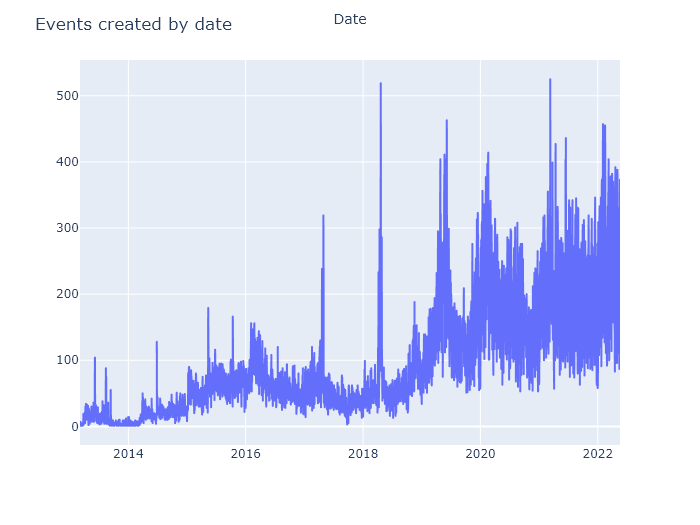
\includegraphics[width=0.99\textwidth]{colab_events_overtime.png}
\end{quadro}

O \autoref{quadro:colab_events_overtime} demonstra a criação de eventos ao longo dos anos. Na imagem pode-se identificar dois picos de mais de 500 postagens por mês: Abril de 2018 e Março de 2022. Além desses picos, é possível observar uma tendência geral de crescimento no número de postagens ao longo dos anos, com algumas flutuações. Por exemplo, em 2017, o número médio de postagens por mês foi de 231, enquanto em 2022, esse número aumentou para uma média de 389 postagens por mês. Isso sugere um aumento no engajamento dos usuários com o aplicativo Colab ao longo do tempo.

Também é interessante notar que o número de postagens tende a aumentar no início do ano, com picos observados em março de cada ano. Isso pode ser devido a fatores sazonais, como o aumento das chuvas no início do ano, que podem levar a mais problemas de infraestrutura urbana sendo relatados.

Em uma análise comparativa dos quatro tipos de interação analisados, observa-se que alguns estão em ascensão, enquanto outros apresentam diminuição na participação. Com o decorrer dos meses, há um aumento no número de curtidas e comentários. Existe uma forte correlação positiva entre a quantidade dessas interações e o tempo decorrido (0,80 para comentários e 0,62 para curtidas). No entanto, o mesmo não ocorre com as conexões e os votos positivos ou negativos nos comentários, que demonstram uma tendência de diminuição no uso. Seria interessante aprofundar a investigação para compreender o motivo dessa queda, especialmente nas conexões, a partir de julho de 2020.

\subsection*{Conexões}

Analisando-se as principais informações sobre a conectividade entre os usuários, isto é, o vínculo entre seguidores e as pessoas que os usuários estão seguindo, tem-se um total de 416.115 ligações. Dentre essas, 402.221 estão ativas e não foram desfeitas (deixar de seguir). As conexões ativas envolvem 112.699 usuários distintos, resultando em uma média de 4,2 conexões e uma mediana de 1 conexão por pessoa. Quanto ao número de seguidores, há variações entre 0 e 854, enquanto o número de pessoas seguidas pelos usuários varia entre 0 e 9.340.

\begin{quadro}[!htb]
	\caption{Distribuição das conexões entre os usuários}
	\label{fig:colab_users_by_connection}
	\centering
	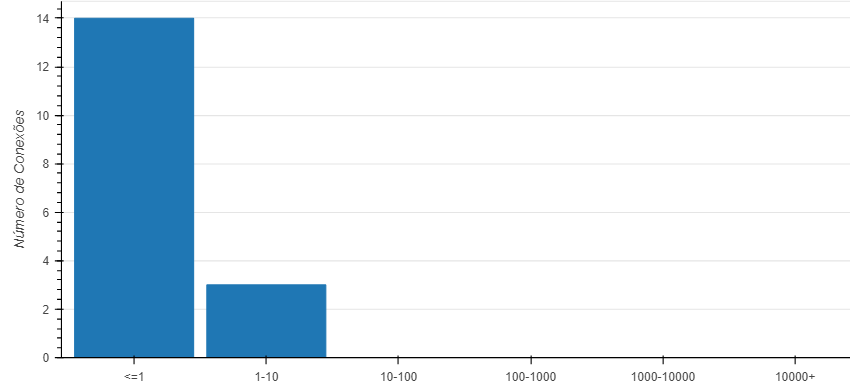
\includegraphics[scale=0.7]{images/colab_users_by_connection.png}
\end{quadro}

Percebe-se que cerca de 83\% dos usuários possuem até 10 conexões, considerando-se a soma de seguidores e pessoas seguidas. Esse valor pode parecer baixo em comparação com outras redes sociais mais populares. No entanto, é importante ressaltar que cada plataforma possui suas particularidades e caberia aprofundar, em estudos futuros, a principal motivação dos usuários para estabelecerem conexões entre si. É possível que muitos usuários busquem se conectar com pessoas conhecidas em seu cotidiano, mas também pode haver usuários que possuam maior influência devido ao seu perfil de uso do aplicativo, por exemplo. Uma outra possibilidade é que alguns usuários não exploram ainda o lado mais social do Colab, o que apresenta-se como uma oportunidade para engajamento. Para compreender se há variações nos perfis de conexões em cada cidade, foram destacadas as informações de Mesquita, Niterói e Santo André.

De maneira geral, Niterói e Santo André apresentam comportamentos semelhantes, com melhor distribuição dos usuários nas faixas de 2-10 e 10-1000 conexões. Nessa última faixa, Niterói possui o maior percentual, com 14\%. Por outro lado, em Mesquita, prevalece a faixa de 1 conexão por usuário (53\%), o que pode indicar uma rede menos integrada (pelo menos em relação às conexões).

\begin{quadro}[!htb]
	\caption{Distribuição das conexões entre os usuários de Mesquita, Niterói e Santo André}
	\label{fig:colab_users_by_connections_on_cities}
	\centering
	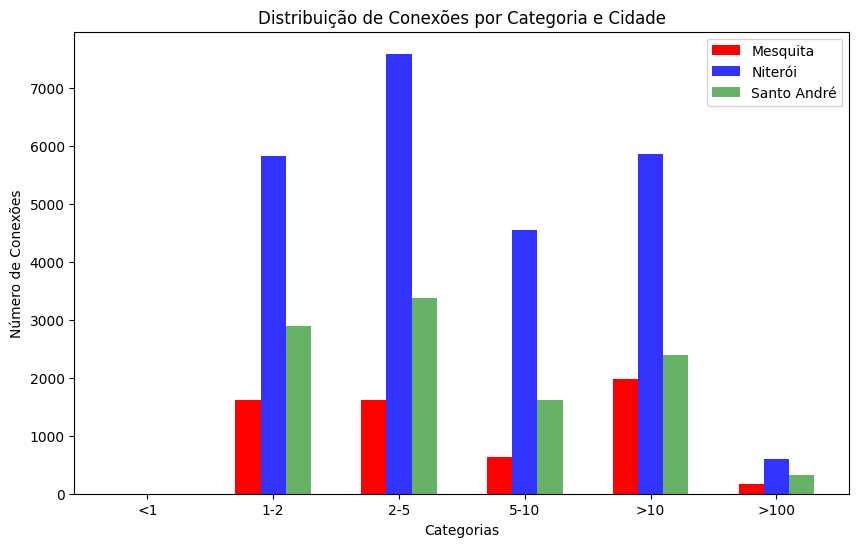
\includegraphics[scale=0.7]{images/colab_users_by_connections_on_cities.png}
\end{quadro}

\subsection*{Apoios}

As curtidas no Colab são divididas em três grandes grupos: curtidas em publicações, comuniques ou propostas (que não existem mais). A plataforma conta com aproximadamente 1,5 milhão de curtidas, realizadas por um total de 100.265 usuários. Verifica-se que a maior parte das curtidas ocorre em publicações relacionadas à zeladoria, as quais representam o maior volume de atividades no feed. Em resumo, a média de curtidas por usuário é de 14, com uma mediana de 2 curtidas. Ao aprofundar a análise para o nível individual dos usuários, é possível constatar diferentes perfis, que variam de 1 até 51.966 curtidas. Apesar de alguns usuários apresentarem um comportamento discrepante, 85\% dos cidadãos realizaram até 10 curtidas. Ao analisar a participação nas três cidades selecionadas - Mesquita, Niterói e Santo André, não foram encontradas diferenças relevantes no percentual de curtidas.

\begin{quadro}[!htb]
	\caption{Distribuição de curtidas ao longo dos anos}
	\label{fig:colab_likes_overtime}
	\centering
	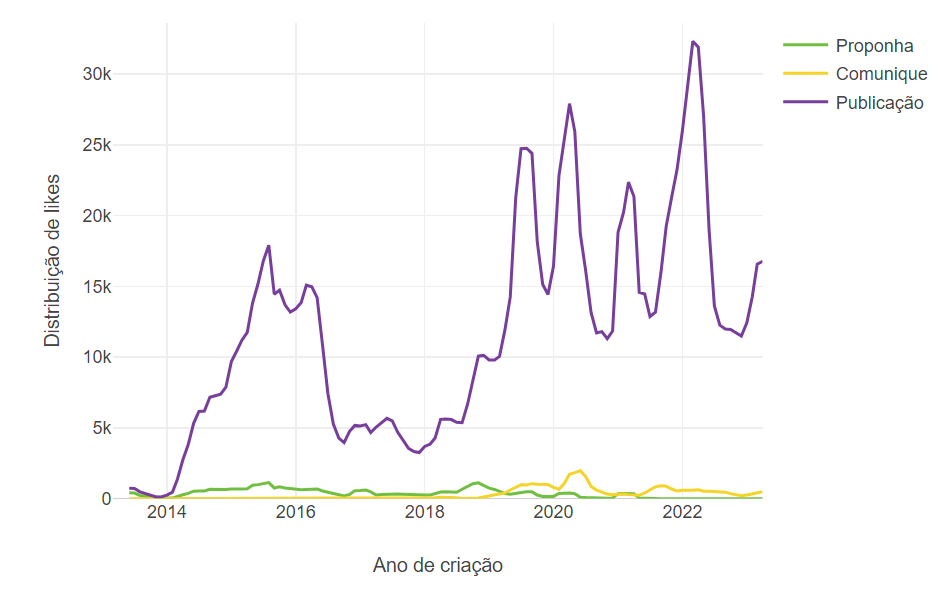
\includegraphics[width=0.9\textwidth]{images/colab_likes_overtime.png}
\end{quadro}

\subsection*{Usuários com mais curtidas}

Ao analisar os usuários com maior número de curtidas, foram destacados os 1.000 usuários que mais curtiram. A faixa etária desses usuários varia entre 13 e 83 anos, com representantes de 62 cidades distintas. As cidades com maior número de representantes são Niterói, Teresina e Juiz de Fora. De maneira geral, predominam pessoas do gênero masculino (71\%), brancos (25\%), com ensino superior completo (35\%) e uma mediana de idade de 44 anos.

\subsection*{Comentários}

Ao analisar os comentários feitos pelos cidadãos, constatou-se a presença de 364.078 comentários até o momento, realizados por 60.452 usuários distintos. Dessa forma, obtemos uma média de 6 comentários por usuário e uma mediana de 2 comentários. O maior número de comentários realizados por um único usuário é de 13.875.Assim como nas conexões e curtidas, a grande maioria dos usuários concentra-se na realização de até 10 comentários.

\begin{quadro}[!htb]
	\caption{Distribuição de comentários por idade}
	\label{fig:colab_comments_by_age}
	\centering
	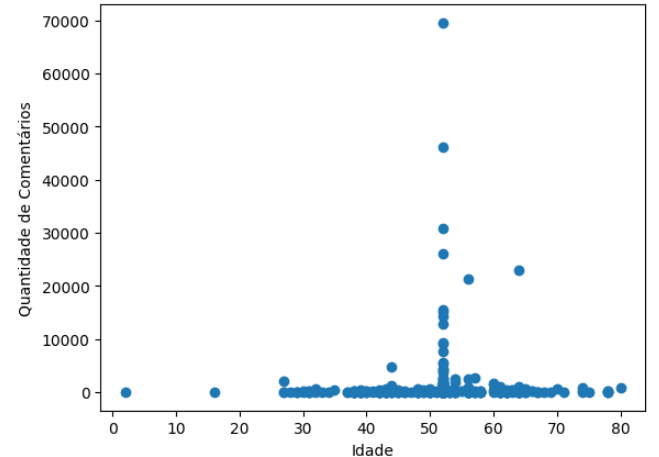
\includegraphics[scale=0.5]{images/colab_comments_by_age.png}
\end{quadro}

Ao isolar as três cidades utilizadas como amostra nesse projeto, podem ser observados comportamentos distintos em cada uma. Nesse caso, Mesquita e Santo André apresentam comportamentos bastante semelhantes, com maior concentração dos usuários na faixa de 1-10 comentários. As três cidades possuem proporções similares nas faixas acima de 10 comentários.

\subsection*{Usuários com mais comentários}

Ao analisar os usuários com maior número de comentários, foram destacados os 1.000 usuários que mais comentam. A faixa etária desses usuários varia entre 16 e 84 anos, com representantes de 51 cidades distintas. As cidades com maior número de representantes são Niterói, Juiz de Fora e Santo André. De maneira geral, há predominância de homens (74\%), brancos (27\%), com ensino superior completo e uma mediana de idade de 45 anos.

\begin{quadro}[!htb]
	\caption{Distribuição de Usuários por Quantidade de Comentários (por Cidade)}
	\label{fig:colab_comments_by_city}
	\centering
	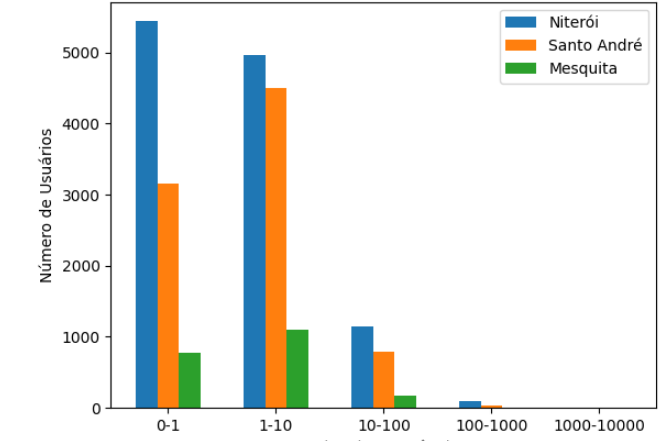
\includegraphics[scale=0.8]{images/colab_comments_by_city.png}
\end{quadro}

\subsection*{Niterói, Mesquita e Santo André}

Para realizar análises mais aprofundadas, tanto de correlações quanto de análises de rede, foram selecionados os dados das três cidades com maior número de interações no Colab: Niterói, Santo André e Mesquita.

\subsection*{Correlação}

Com o objetivo de traçar um perfil dos usuários mais ativos na plataforma, buscou-se identificar alguma correlação entre a quantidade de atividades realizadas pelos cidadãos e suas principais características cadastrais (quando disponíveis).

\begin{quadro}[!htb]
	\caption{Matriz de Correlação}
	\label{fig:colab_correlation_matrix}
	\centering
	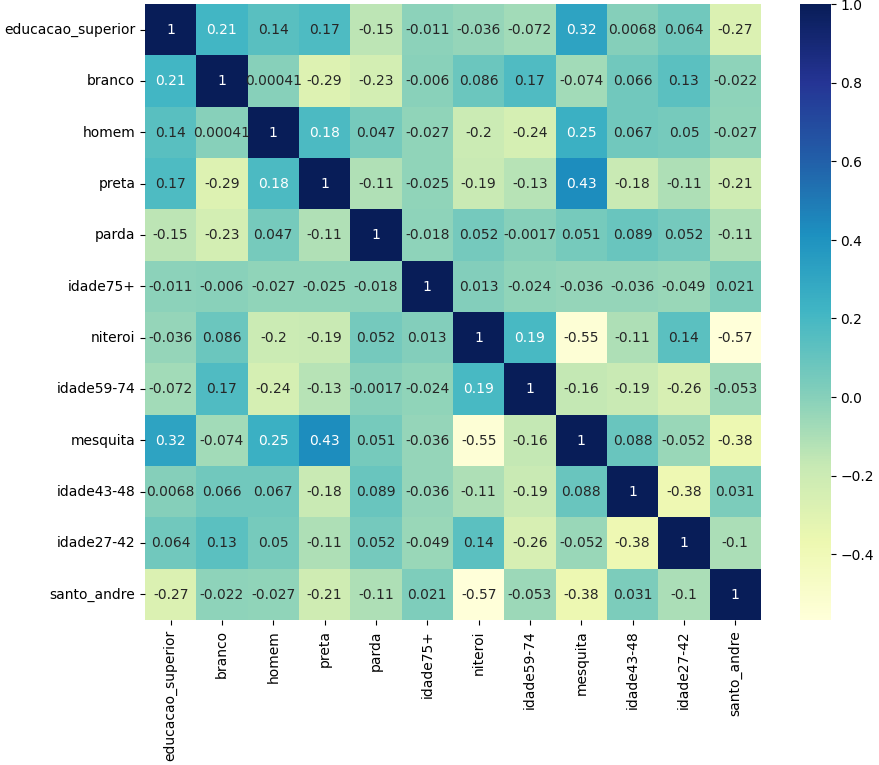
\includegraphics[scale=0.6]{images/colab_correlation_matrix.png}
\end{quadro}

Para viabilizar a análise, algumas características foram transformadas em formato booleano (TRUE/FALSE). As características utilizadas foram:

\begin{itemize}
	\item Cidade do usuário, com destaque para Mesquita, Niterói e Santo André.
	\item Escolaridade, sendo considerado o nível "Superior +" que engloba ensino superior completo, mestrado e doutorado.
	\item Idade, considerada no intervalo de 10 a 90 anos e segmentada em cinco faixas etárias. Para a segmentação, adotou-se o método de passos iguais, no qual cada faixa representa um intervalo igual de anos. As faixas etárias definidas foram: 10-26; 27-42; 43-58; 59-74; 75-90.
	\item Tipos de interações considerados para análise: comentários em publicações, curtidas em publicações, seguidores/seguindo e endosso ou rejeição de comentários .
	\item Cor/raça, incluindo as categorias branca, preta e parda.
	\item Gênero, considerando apenas homens.
	\item Número de interações acima da mediana do total de interações de cada usuário.
\end{itemize}

A expectativa inicial era que determinadas características, como escolaridade avançada ou faixa etária específica, pudessem indicar um padrão de maior envolvimento cívico. No entanto, a ausência de correlações significativas sugere que a participação na plataforma Colab pode ser mais influenciada por fatores não capturados pelos dados demográficos ou pelo registro de interações disponíveis.

Essa falta de correlações fortes tem várias implicações para a pesquisa:

\begin{itemize}
	\item \textbf{Diversidade de Engajamento:} A participação cívica na plataforma Colab pode ser mais heterogênea do que inicialmente previsto, com um amplo espectro de cidadãos se engajando por motivos diversos e contextuais.
	\item \textbf{Influência de Fatores Exógenos:} Fatores externos à plataforma, como campanhas de conscientização, eventos locais ou nacionais, e movimentos sociais, podem ter um papel mais significativo no direcionamento da participação dos usuários.
	\item \textbf{Necessidade de Dados Mais Profundos:} Para uma compreensão mais completa do engajamento dos usuários, seria útil ter acesso a dados mais detalhados sobre suas motivações, percepções e a qualidade das interações, além das métricas quantitativas. Isso poderia ser obtido por meio do recurso de \textit{Consultas} do Colab, que esclarece a opinião dos usuários através de enquetes rápidas, mas esses dados estão indisponíveis para análise.
	\item \textbf{Amplitude do Design de Pesquisa:} Este achado aponta para a necessidade de abordagens de pesquisa mais granulares, analisando correlações em comunidades locais em vez de em todo a rede, e considerando fatores exógenos que podem influenciar o engajamento.
\end{itemize}

O desafio subsequente será identificar métodos e fontes de dados que possam revelar os fatores subjacentes que impulsionam a atividade no app, que, por sua vez, poderia informar estratégias para aumentar o engajamento e a eficácia das iniciativas da plataforma.

\begin{figure}[!htb]
	\caption{Matriz de Correlação}
	\label{fig:colab_correlation_bingo}
	\centering
	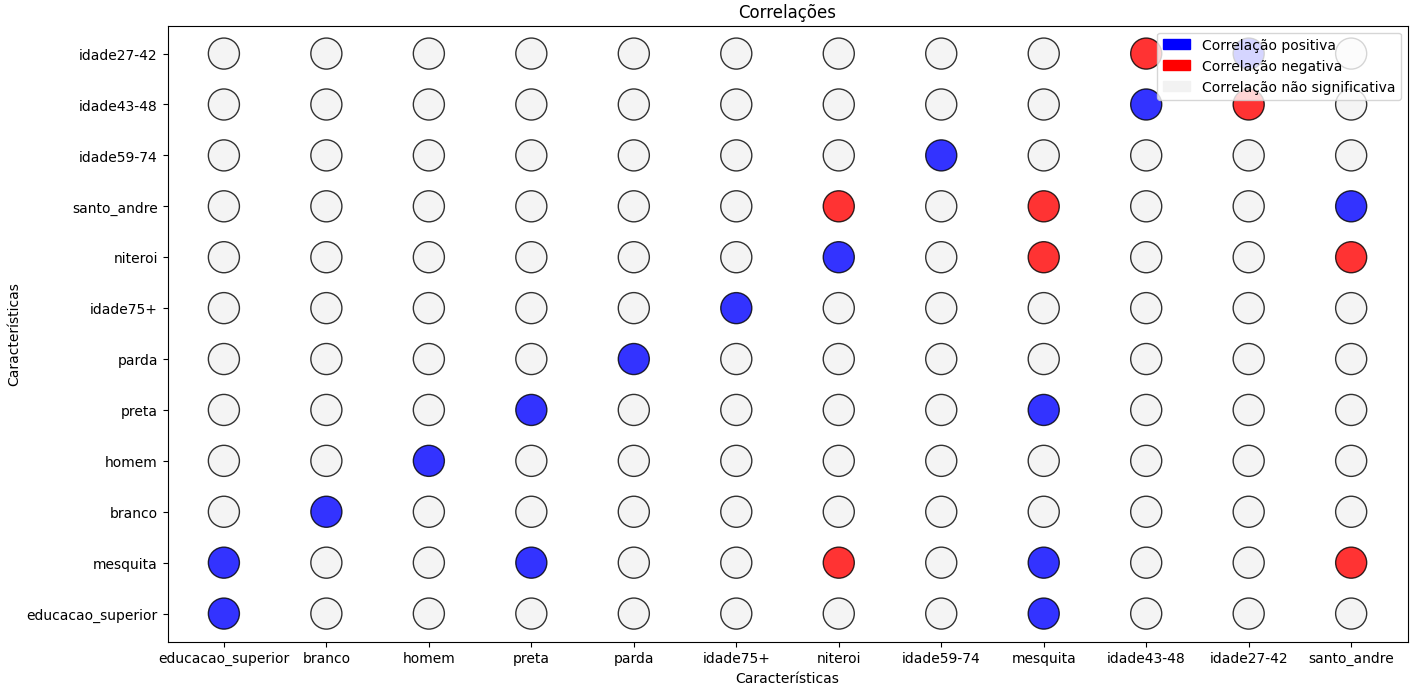
\includegraphics[scale=0.4]{images/colab_correlation_bingo.png}
\end{figure}

\subsection*{Regressão Logística}

A análise comportamental dos usuários do Colab foi aprofundada através da aplicação de um modelo de regressão logística \cite{2010_Yu} utilizando a biblioteca Scikit-learn \cite{2011_Pedregosa}. Esta técnica estatística permite estimar a probabilidade da ocorrência de um evento, neste caso, um alto nível de interações na plataforma (mais de 3 interações, acima da mediana), baseando-se em várias características dos usuários.

As variáveis preditoras selecionadas foram aquelas que representam as características demográficas e de engajamento dos usuários. A variável dependente foi binarizada, com o valor TRUE indicando usuários altamente ativos e FALSE para aqueles menos ativos, conforme a mediana de interações.

\begin{quadro}[!htb]
	\caption{Curva ROC da Regressão Logística}
	\label{fig:regression_roc}
	\centering
	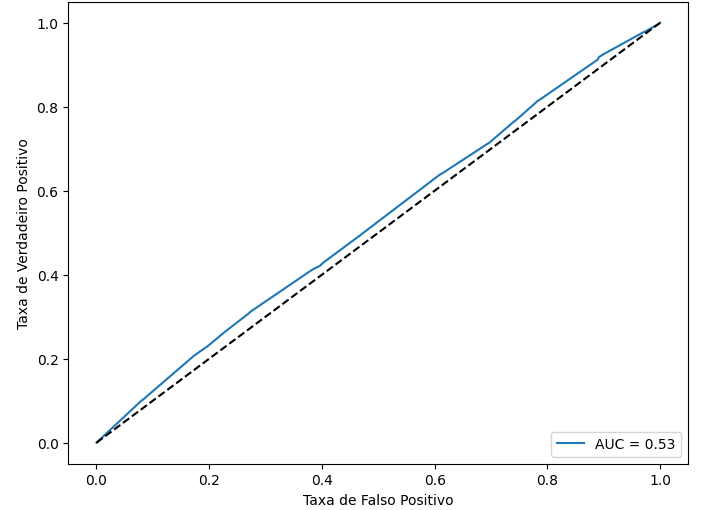
\includegraphics[scale=0.8]{images/regression_roc.png}
\end{quadro}

Primeiramente, identificamos e lidamos com o desbalanceamento no conjunto de dados, aplicando a técnica de oversampling através do Synthetic Minority Over-sampling Technique (SMOTE). Isso ajudou a criar um conjunto de dados mais equilibrado, garantindo que o modelo não fosse enviesado para a classe majoritária. Em seguida, aprimoramos o modelo substituindo a regressão logística pelo algoritmo XGBoost, que é mais robusto e adequado para capturar interações complexas entre features. Adicionalmente, realizamos uma otimização de hiperparâmetros utilizando uma busca em grade (GridSearchCV) para encontrar os melhores valores de parâmetros como 'learning rate', 'max depth' e 'number of estimators'. Essas modificações culminaram em uma melhora significativa na performance do modelo, resultando em uma AUC de 0.78. Esse aumento na AUC indica que o modelo agora é muito mais eficaz em distinguir entre os diferentes níveis de atividade dos usuários na plataforma, refletindo uma capacidade aprimorada de prever comportamentos um pouco mais complexos. Dentre as variáveis analisadas, as seguintes mostraram-se mais relevantes para o modelo:

\begin{quadro}[!htb]
	\caption{Curva ROC da Regressão Logística}
	\label{fig:xgb_roc}
	\centering
	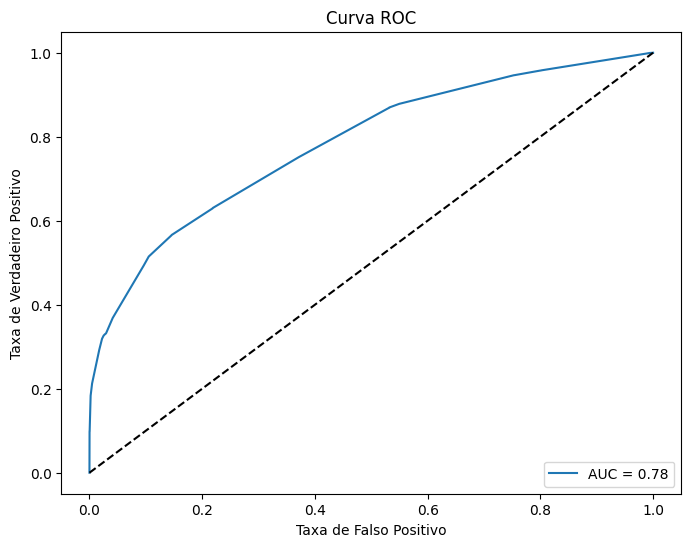
\includegraphics[scale=0.8]{images/xgb_roc.png}
\end{quadro}

\begin{itemize}
	\item Residência na cidade de Niterói, o que pode indicar diferenças culturais ou sociais regionais que impactam o engajamento na plataforma.
	\item A autodeclaração da cor branca, que levanta questões sobre a representatividade e o acesso à plataforma em diferentes grupos étnicos.
	\item Níveis de escolaridade superior, sugerindo que um maior nível educacional pode estar associado a um maior envolvimento cívico online.
	\item A autodeclaração da cor parda, que, junto à variável da cor branca, sinaliza a necessidade de investigar mais a fundo as dinâmicas raciais na participação da plataforma.
	\item Gênero masculino, indicando potenciais disparidades de gênero no engajamento com o Colab.
\end{itemize}

\begin{quadro}[!htb]
	\caption{Coeficientes da Regressão Logística}
	\label{fig:regression_chart}
	\centering
	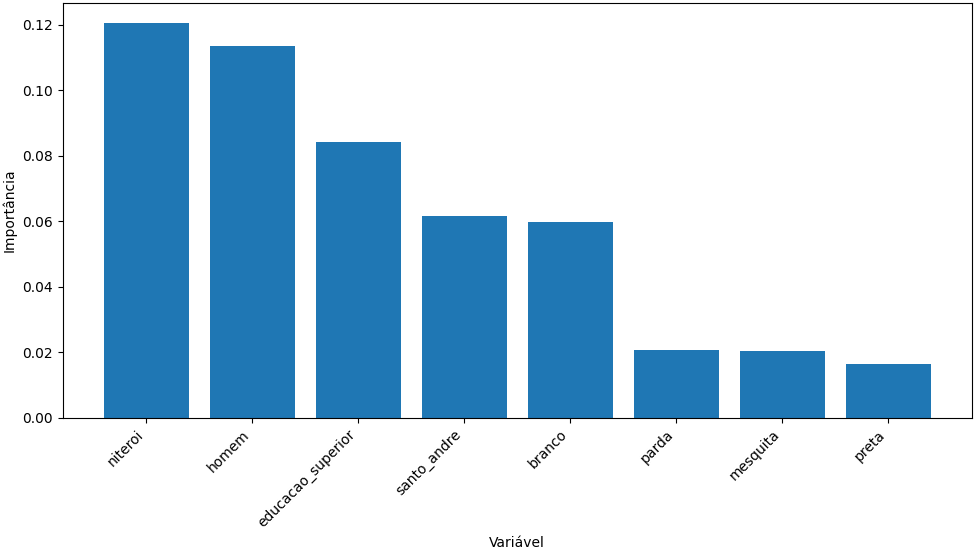
\includegraphics[scale=0.6]{images/regression_chart.png}
\end{quadro}

Apesar da previsibilidade inicial relativamente baixa, o aprimoramento do modelo de AUC de 0.52 para 0.78 é um avanço significativo. Esse progresso sublinha a importância de identificar e ajustar as variáveis preditoras corretamente, produzindo dados sobre as características demográficas que influenciam o uso da plataforma. A análise dessas variáveis destaca a necessidade de considerar a inclusão e a diversidade no design de sistemas Gov-Tech. Pretendemos utilizar as features mais relevantes identificadas para aprimorar a segmentação de grupos de usuários selecionados para uma análise mais específica. O foco nas 3 cidades de Niterói, Mesquita e Santo André parece evidente, assim como as disparidades de gênero e escolaridade. Este avanço sugere que a combinação de técnicas de balanceamento de dados e tuning de hiperparâmetros pode ser uma abordagem eficaz para melhorar ainda mais a performance do modelo e fornecer insights mais precisos para intervenções futuras.

\section{Conclusões}
Neste capítulo, exploramos em detalhes o cenário do Colab, uma plataforma que desempenha um papel fundamental na conexão entre os cidadãos e suas autoridades municipais, proporcionando uma interface direta para relatórios de problemas urbanos e interações com a administração pública. Ao longo deste capítulo, analisamos o histórico do Colab e como a plataforma evoluiu ao longo dos anos, crescendo em termos de engajamento dos usuários e na variedade de problemas urbanos relatados. Observamos dois picos notáveis de atividade em 2018 e 2022, sinalizando um aumento constante na conscientização e no uso da plataforma.

Além disso, discutimos como o Colab serve como uma interface crucial para a resolução de problemas urbanos. Os dados revelam que a plataforma é frequentemente usada para relatar questões relacionadas à infraestrutura urbana, como buracos nas estradas e entulho nas calçadas, destacando sua importância na vigilância participativa e na melhoria da qualidade de vida nas cidades. A análise das conexões entre os usuários do Colab também fornece insights sobre como a comunidade interage e se relaciona, mostrando a diversidade de perfis e comportamentos.

As descobertas deste capítulo oferecem várias implicações práticas para o aprimoramento da vigilância participativa e para políticas de gestão pública mais inclusivas e eficazes. A análise dos padrões de interação e comportamento dos usuários no Colab fornece uma base de conhecimento que pode ser utilizada para fomentar uma cidadania mais ativa e responsiva. A identificação de características demográficas associadas a um maior engajamento na plataforma Colab sugere a necessidade de políticas de inclusão digital que abordem as disparidades existentes. Isso pode incluir a criação de programas educativos que incentivem o uso de plataformas Gov-Techs por grupos sub-representados e a adaptação de interfaces para torná-las mais acessíveis a uma gama mais ampla de usuários.

As variáveis demográficas relevantes, como localidade, raça e gênero, destacam a necessidade de uma abordagem mais equitativa na vigilância participativa. Estratégias para promover a participação equitativa podem incluir campanhas de conscientização focadas em comunidades específicas e a formação de parcerias com organizações locais para alcançar uma base de usuários mais diversificada. Além disso, a análise de redes pode ser usada para identificar usuários influentes e líderes de opinião que podem ser mobilizados para promover a participação de grupos sub-representados.

Os insights obtidos através da análise de dados do Colab podem informar a elaboração de políticas públicas que respondam melhor às necessidades dos cidadãos. A vigilância participativa, fortalecida por uma compreensão profunda do comportamento dos usuários, pode levar a intervenções mais direcionadas e efetivas, melhorando a prestação de serviços públicos e a qualidade de vida dos cidadãos.

No próximo capítulo, avançaremos na pesquisa ao apresentar uma análise exploratória das redes, buscando identificar e refinar ainda mais os padrões de conexões, influências e clusters de usuários, contribuindo para uma visão mais completa e detalhada da dinâmica de redes no aplicativo com a inteção de isolar comunidades que possam se comportar como câmaras de eco ou ambientes de alta polarização.